\section{LCD}
\textbf{Sicherheitshinweis:} Vorsicht beim Umgang mit den Chemikalien und immer eine Schutzbrille tragen.\\
\subsection{Funktionsweise}

\begin{figure}[t]
  \centering
  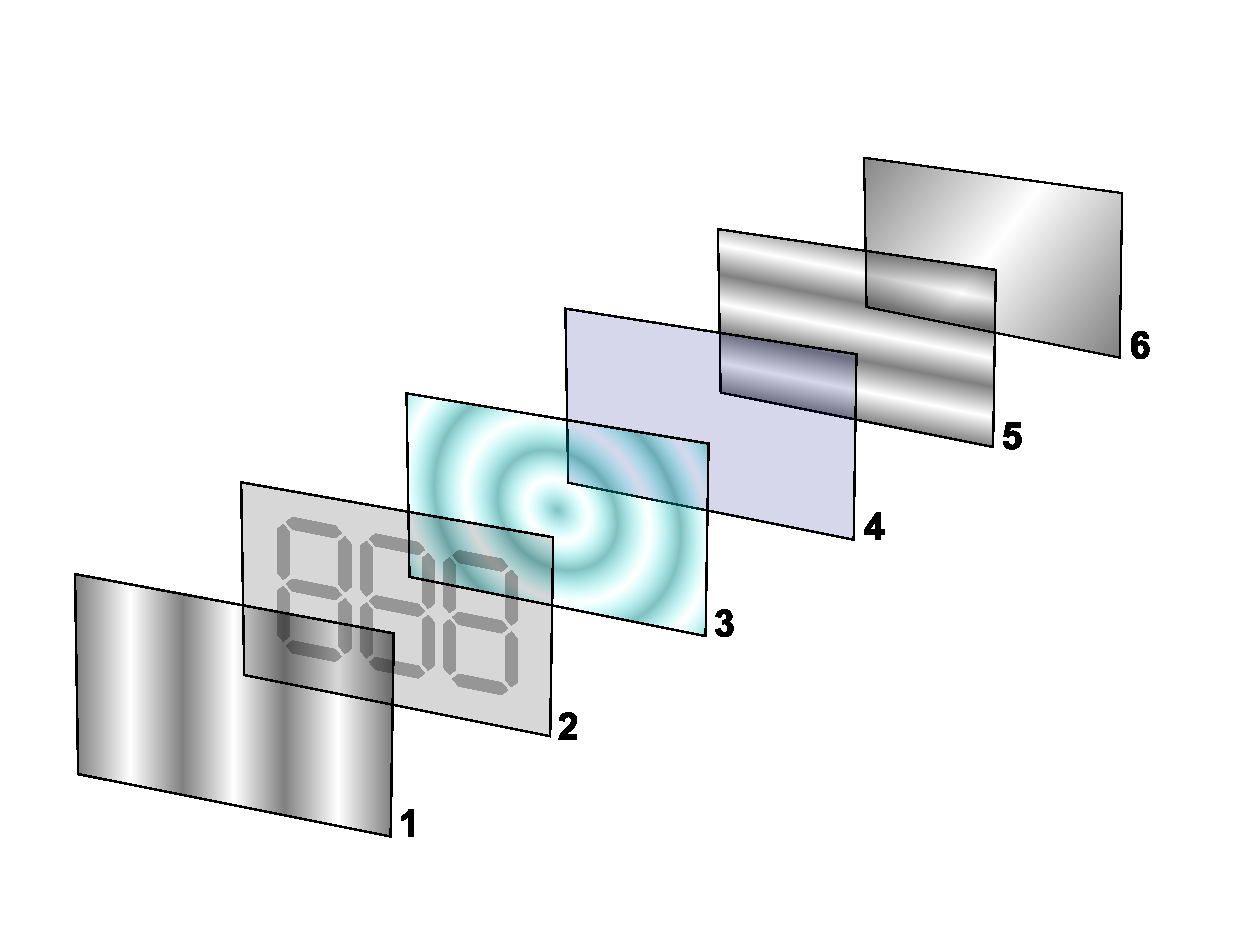
\includegraphics[width=\linewidth, keepaspectratio]{Bilder/LCD_layers}
  \caption{Aufbau eines LCDs mit Polarisationsfolien (Markierung 1 und 5), zwei beschichteten, leitenden Glasplatten (Markierung 2 und 4), den Flüssigkristallen (Markierung 3) und einem Reflektor (Markierung 6) nach ref[FIXME REF]}
  \label{lcdaufbau}
\end{figure}

Das Display besteht aus zwei zusammengeklebten Glasplatten mit einem Abstand von circa 10 Mikrometern. Auf den Glasplatten befinden sich leitende Schichten aus Indium-Zinn. Diese Schichten werden später zur Darstellung von Zeichen oder Symbolen verwendet. Der grundsätzliche Aufbau eines LCD Displays besteht aus folgenden Teilen (siehe Abbildung \ref{lcdaufbau}):
\begin{itemize}
\item Zwei Glasplatten, die mit der leitenden Schicht überzogenen Innenseiten liegen sich gegenüber (Markierung 2 und 4)
\item Zwischen den Glasplatten: Flüssigkristall (Markierung 3)
\item Außerhalb der Glasplatten: Polarisationsfolienn (Markierung 1 und 5)
\item Eine Refelektorfolie auf einer Seite (Markierung 6)
\end{itemize}
Die Glasplatten werden so präpariert, dass die zigarrenförmige Moleküle auf jeweils einer Glasplatte in eine Richtung zeigen. Auf der gegenüberliegenden Seite sind sie um 90 Grad gedreht. Der Flüssigkristall beschreibt eine “Schraubenstruktur”. Diese verschraubte Struktur veranlasst polarisiertes Licht, ihr zu folgen. Ohne Spannung wird die Polarisationsebene um 90 Grad gedreht und das Licht wird durchgelassen und reflektiert. Beim Anlegen von Spannung (ca. 3V Wechselspannung -> siehe Kapitel \ref{sec:elektronik}) richten sich die Moleküle kollektiv senkrecht zu den Elektroden aus. Somit existiert also für das Polarisationslicht keine Schraubenstruktur mehr. Folglich wird beim Durchgang durch die Zelle der Polarisationszustand nicht beeinflusst, was schließlich dazu führt, dass die Bereiche dunkel erscheinen (Quellen: \cite[Bauanleitung]{Bauanleitung} \cite[LCD Aufbau und Funktion]{aufbau_und_funktion})


%\subsection{Produktionsschritte}
%\textbf{Schritt 1:} Strukturierung der Elektroden, durch Aufbringen der Klebefolie auf die Bereiche, an denen ein Symbol sichtbar sein soll.\\
%\textbf{Schritt 2:} Wegätzen der beschichteten Bereiche, die nicht angezeigt werden sollen (mit 5\% Salzsäure), sodass die braune leitende Indium-Zinn Schicht der Glasplatten verschwindet.\\
%\textbf{Schritt 3:} Entfernen der Abdeckschicht (Klebefolie), dabei werden Klebereste mit Aceton entfernt.\\
%\textbf{Schritt 4:} Oxidieren der Indium-Zinn-Schicht (im Ofen bei 250 Grad) zu Indium-Zinn-Oxid, damit die Glasplatten möglichst transparent werden und noch leitfähiger werden.\\
%\textbf{Schritt 5:} Reinigung der Glasplatten durch Kochen in einem im Verhältnis 1:5 verdünnten alkalischen tensidfreien Reinigungsbad für 5 Minuten, damit die Glasplatten komplett fettfrei werden. Dabei werden auch Siedesteinchen verwendet, um einen Siedeverzug zu vermeiden.\\
%\textbf{Schritt 6:} Orientierung der Oberflächenmoleküle der leitenden Schicht der Glasplatten durch die sogenannte {\quote Reiborientierung}. Dies geschieht mit Hilfe eines Zellstofftuchs mit dem über die Platten gerieben wird. Die obere und die untere Glasplatte müssen 90 Grad versetzt orientiert sein.\\
%\textbf{Schritt 7:} Zwischen den Glasplatten werden am Rand Abstandshalter eingelegt, damit diese sich später mit einem Abstand von ungefähr 12 Mikrometern  gegenüberliegen. Hier eignet sich zum Beispiel die Verpackungsfolie von Zigarettenschachteln.\\
%\textbf{Schritt 8:} Die Glasplatten werden mit übereinandergelegt, sodass sich die beiden leitenden Seiten gegenüberliegen. Danach werden zunächst zwei parallele Seiten mit einem Zweikomponent-Kleber verklebt, während Druck auf die Abstandhalterfolie ausgeübt wird. Dadurch wird gewährleistet, dass der Abstand bewahrt wird. Ansonsten zeigt die Zelle später eine langsamere elektrooptische Reaktion. \\
%\textbf{Schritt 9:} Nun werden Tropfen des  Flüssigkristalls an die noch offene Kanten gesetzt, und der Flüssigkristall zieht selber durch die Kapillarwirkung in die Zelle ein. Anschließend werden die noch offenen Kanten mit dem Kleber verschlossen.
%(Quelle: \cite[Bauanleitung]{Bauanleitung})

\subsection{Elektrodenstrukturaufbringung}

In diesem Kapitel wird beschrieben, wie die gewünschten Strukturen auf die leitend beschichteten Glasplatten aufgebracht werden können. Hierfür kommen 3 Methoden in Betracht. Mittels eines fotosensitiven Lacks, Folien aus dem Folienplotter des FAUFabLab oder per Edding.\\

\subsubsection*{Fotolack}

Wie bei der Herstellung von Platinen wird auf die leitende Seite der Glasplatten eine Schicht Fotolack aufgetragen. Verwendet wurde \cite[\textit{POSITIV 20 Lichtemfpindlicher Lack}]{Fotolack}.
Bei Raumtemperatur muss der Lack für 24h an einem dunklen Ort trocknen. Die Glasplatten sollten zudem vor dem Besprühen gut gereinigt werden, um Fettflecken und andere Verunreinigungen zu entfernen. Ansonsten besteht die Gefahr, dass der Lack nicht gut haftet oder sich schlecht verteilt.
Auf mehreren Platten wurde der Fotolack in verschiednene Arten aufgetragen. Zum einen wurde ein Test für 1 bis zu 5 aufgetragenen Schichten durchlaufen. Des Weiteren wurden die Platten flach auf dem Boden liegend, sowie in einem 30 Grad Winkel besprüht.
Mit letzerer Methode wurde das beste Ergebnis erzielt, da der Lack leicht nachlfließen konnte und sich somit am schönsten verteilt hat. Bei der Schichtdicke war es ausreichend eine einzelne Schicht aufzutragen.

Nun werden die beschichteten Glasplatten in den Belichter gelegt und das Anzeigedesign, welches auf Papier ausgedruckt wurde, auf die beschitete Seite gelegt. Wie beim Belichten von Platinen ist eine Belichtungszeit von 9:40 min zu wählen. Da es sich um Glasplatten handelt, auf denen von beiden Seiten Licht durchdringen kann, ist umbedingt darauf zu Achten ein lichtundruchlässiges Objekt auf die nicht mit Fotolack beschichtete Seite zu legen (Beispielsweise eine schwarze Acrylplatte). Ansonsten wird die komplette Fotolackschicht belichtet. Anschließend wird der Fotolack entwickelt (NaOH, siehe Abschnitt \ref{subsec:platine}).\\


\begin{figure}[t]
  \centering
  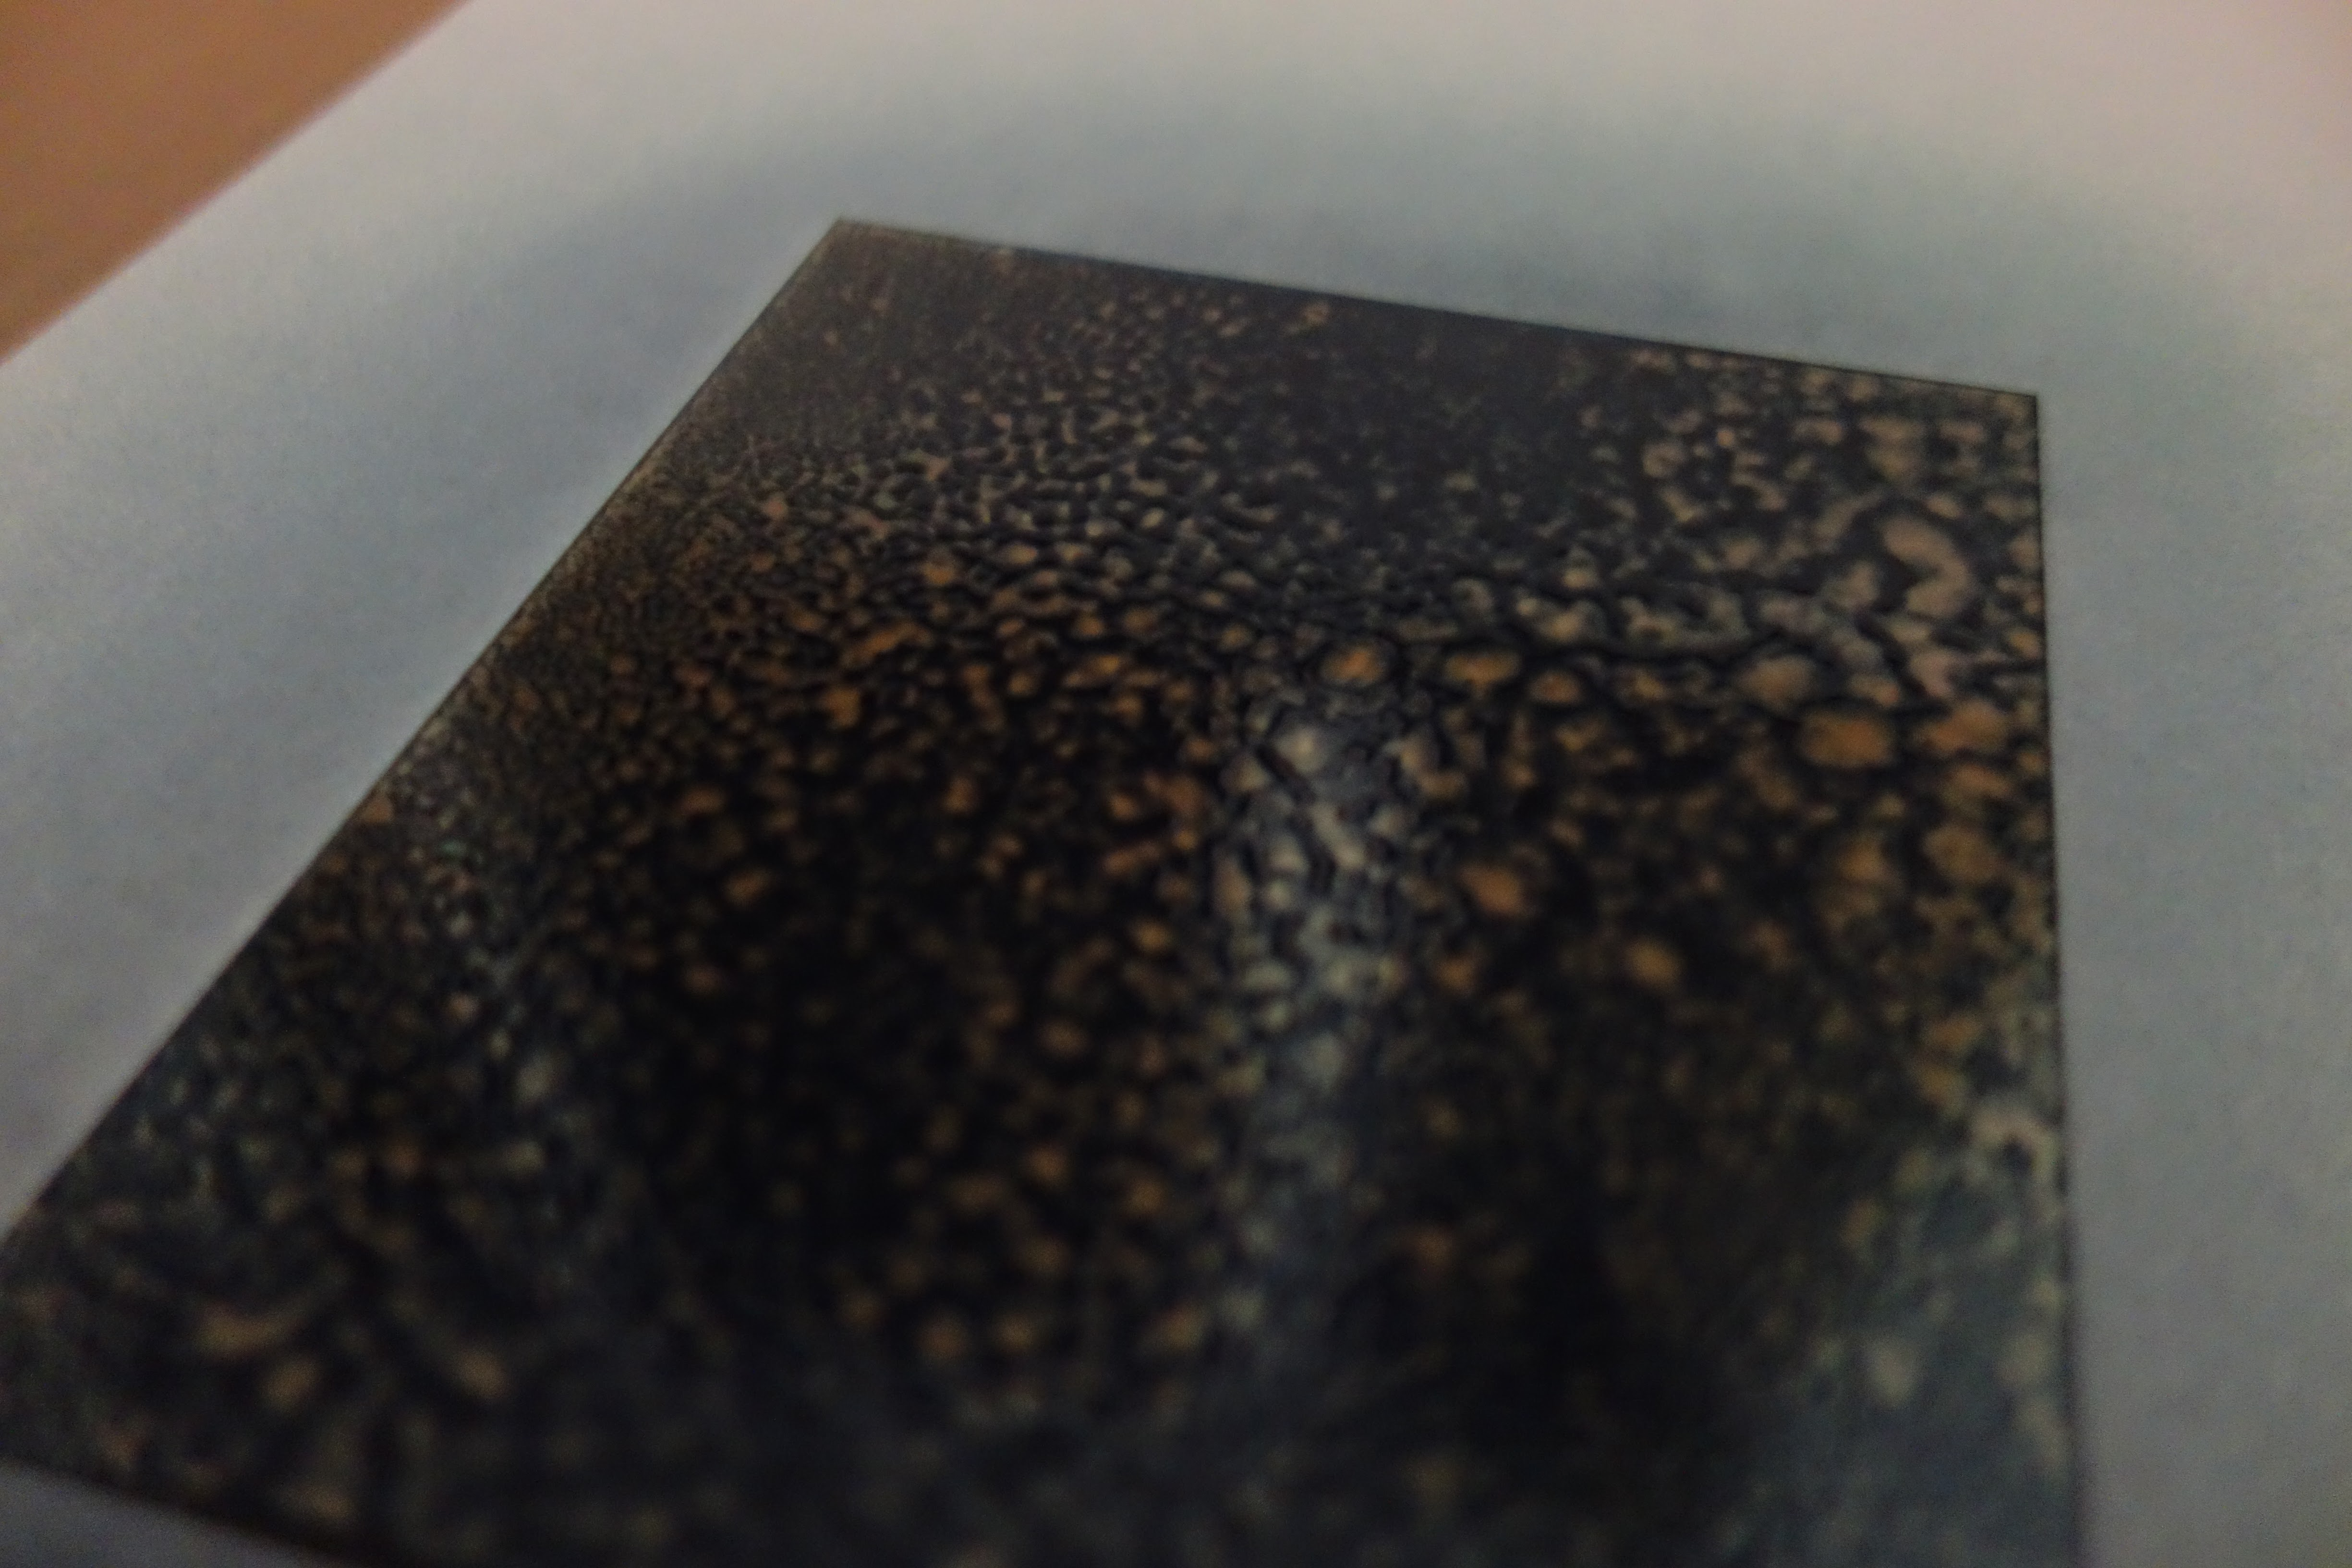
\includegraphics[height=0.2\textwidth, keepaspectratio]{Bilder/Fotolackverfahrenbeschichtet}
  \caption{Mit Fotolack beschichtete Glasplatte}
  \label{Fotolackbeschichtete Glasplatte}
\end{figure}

\begin{figure}[t]
  \centering
  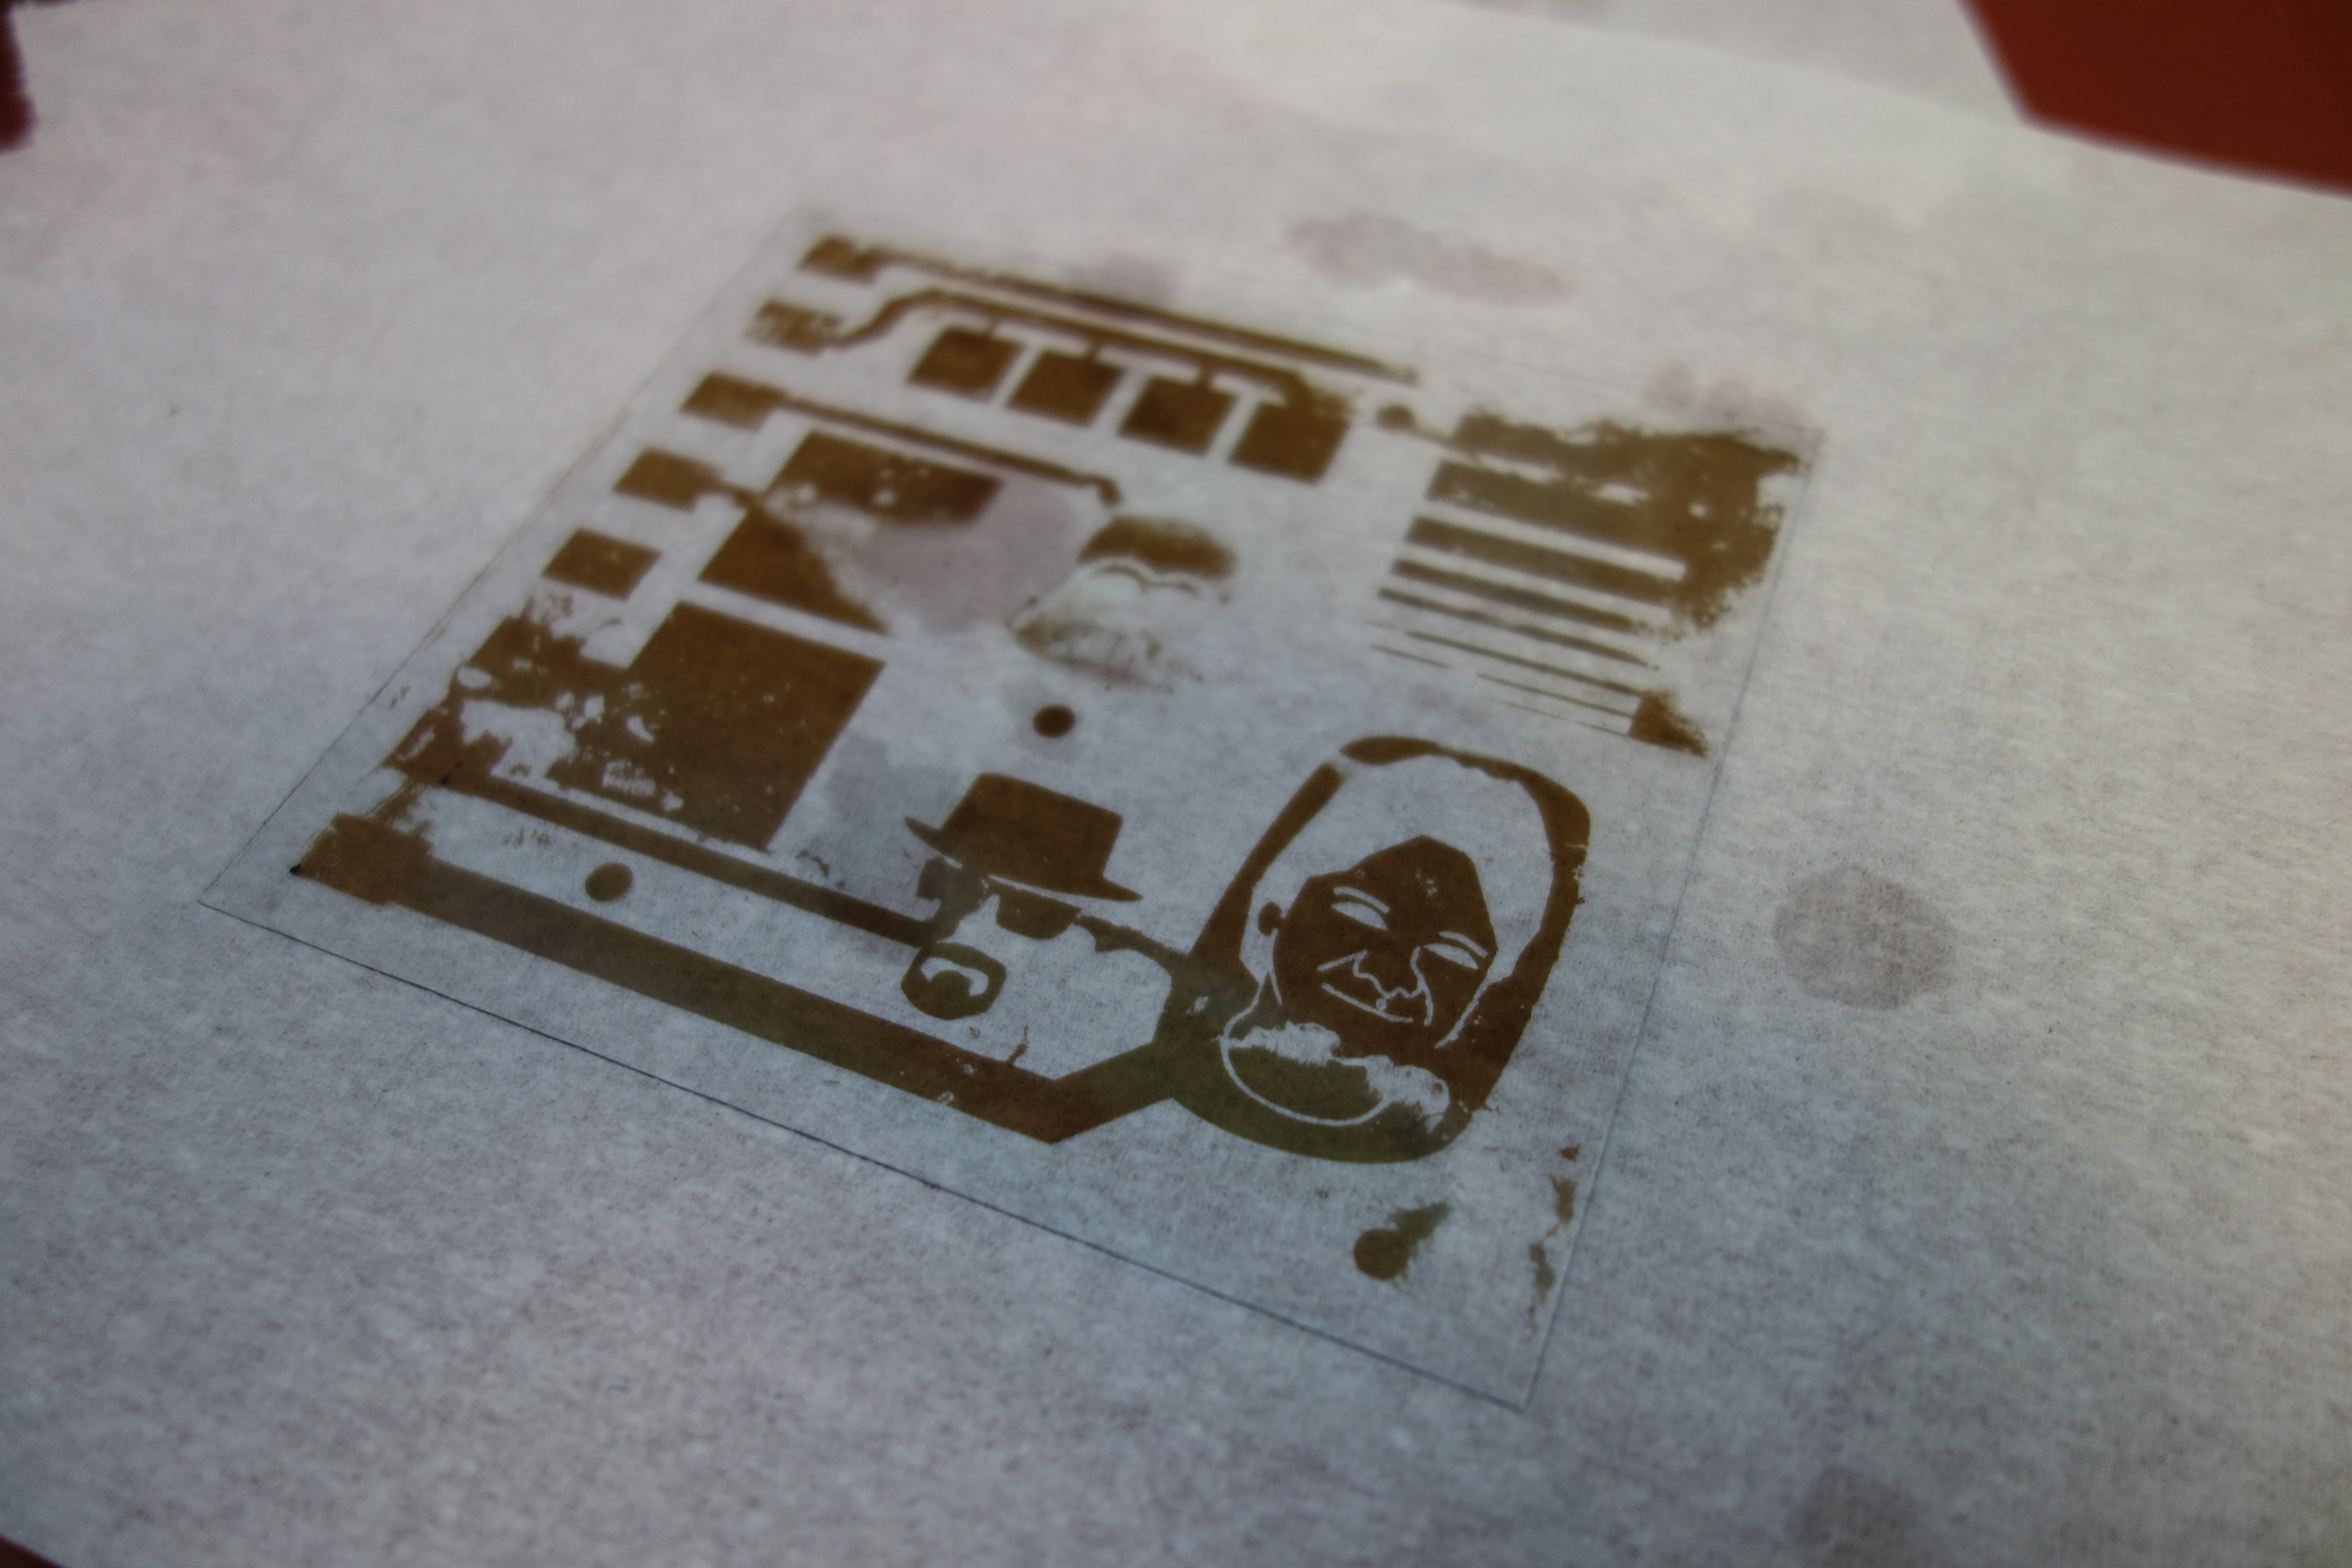
\includegraphics[height=0.2\textwidth, keepaspectratio]{Bilder/Fotolackverfahrengeaetzt}
  \caption{Fotolackverfahren Aetzung}
  \label{Fotolackverfahren Aetzung}
\end{figure}

\subsubsection*{Klebefolie}\label{subsec:klebefolie}
Muster werden entworfen und mit einem Plotter aus einer selbstklebenden Klebefolie ausgeschnitten. Das Muster wird auf einer Übertragungsfolie aufgebracht und auf die leitende Schicht der Glasplatten aufgeklebt, anschließend wird die Übertragungsfolie abgezogen. Nun sind alle Stellen, die später leuchten sollen, abgedeckt. Versuche haben bestätigt, dass die Klebefolie die leitende Indium-Zinn Schicht nicht entfernt oder merklich schädigt. Die Vorteile der Folie sind, dass komplexe Strukturen hergestellt werden können und sehr scharfe Kanten entstehen. Allerdings ist das anschließende Abziehen der Folie sehr mühsam.
Es lässt sich festhalten, dass das Endergebnis bei der Beschichtung mit Fotolack nicht zufriedenstellend ist. Es hat sich als Schwierig erwiesen den Lack gleichmäßig aufzubringen, sodass beim Entwickeln und Ätzen alle Stellen gleichmäßig mit dem Chemikalien behandelt werden. Das Endergebnis ergab ein sehr unscharfes Bild, weshalb sich diese Methode als ungeeignet erwies.\\

\subsubsection*{Edding}
Weitere Möglichkeiten zur Elektrodenstrukturierung sind mit Hilfe eines wasserfesten Edding Strukturen direkt aufzumalen. Diese Verfahren sind zwar einfacher, allerdings entstehen hierbei keine so scharfen Kanten wie durch eine Folie entstehen und keine sauberen Strukturen abgebildet werden können.\\

Wegen der oben genannten Gründe greifen wir für die Herstellung unseres Displays auf die Methote Folienplott zurück.


\subsection{Ätzen der Struktur}
%\textbf{Sicherheitshinweis:} Vorsicht beim Umgang mit den Chemikalien und immer eine Schutzbrille tragen.\\

Um die Elektroden freizulegen muss an allen Stellen, an denen das Display nichts anzeigen soll die leitende Schicht weggeätzt werden. Dies ist daran zu erkennen, dass die brauen Färbung der leitenden Indium-Zinn Schicht vollständig verschwindet. Hierbei stehen zwei Verfahren zur Auswahl.\\

\subsubsection*{Salzsäure}

Zum Einen lässt sich die Indium-Zinn-Schicht sehr schnell und einfach mit Salsäure (5\%) entfernen. Hierfür wird die Glasplatte mit der schützenden Schicht, (Fotolack, Klebefolie oder Edding) in Salzsäure gelegt. Bereits nach 30 sek ist der Vorgang beendet. Gegenenfalls können die Platten auch länger im Salsäurebad verweilen. Dies könnte allerdings dazu führen, dass die Salzsäure unter die Klebefolie zieht und zu viel wegätzt.\\

\subsubsection*{Platinenätzmittel}
Das Wegätzen der Indium-Zinn Schicht ist auch durch das Ätzbad (Natriumpersulfatlösung) möglich, welches im FAUFabLab zum Ätzen von Platinen verwendet wird. Dazu wird eine Natriumpersulfatlösung verwendet und nach ca. 20 Minuten war bei unserem Versuch die leitende Indium-Zinn-Schicht entfernt. Diese Methode stellt also eine gute Alternatie zur Salzsäure dar.\\

\begin{figure}[t]
  \centering
  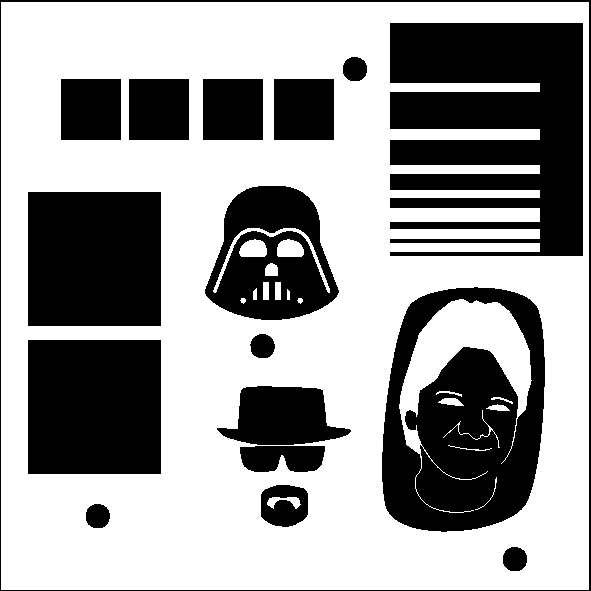
\includegraphics[width=0.5\linewidth, keepaspectratio]{Bilder/testmuster}
  \caption{Testmuster (Anzeigen und Ausrichtungspunkte)}
  \label{testmuster}
\end{figure}


\begin{figure}[t]
  \centering
  \subfigure[Testmuster (Anzeigen, Ausrichtungspunkte und Zuleitungen untere Seite)]{
  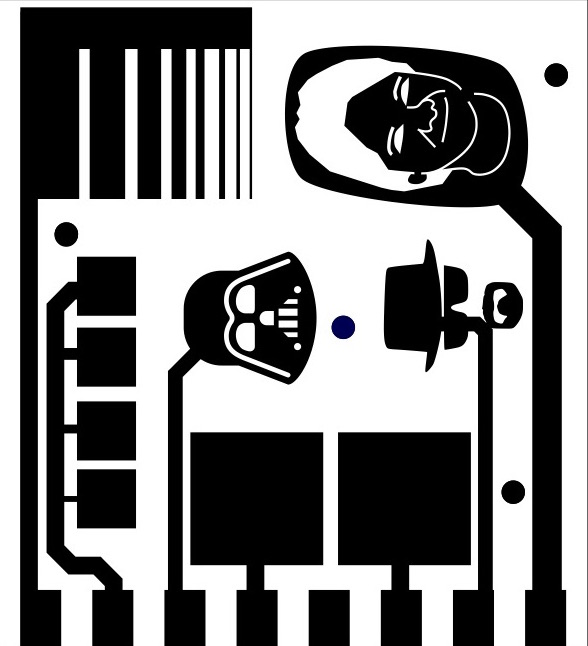
\includegraphics[height=0.2\textwidth, keepaspectratio]{./Bilder/testmuster-seite1.jpg}
  \label{testmuster-seite1}
}
~
\subfigure[Testmuster (Anzeigen, Ausrichtungspunkte und Zuleitungen obere Seite)]{
  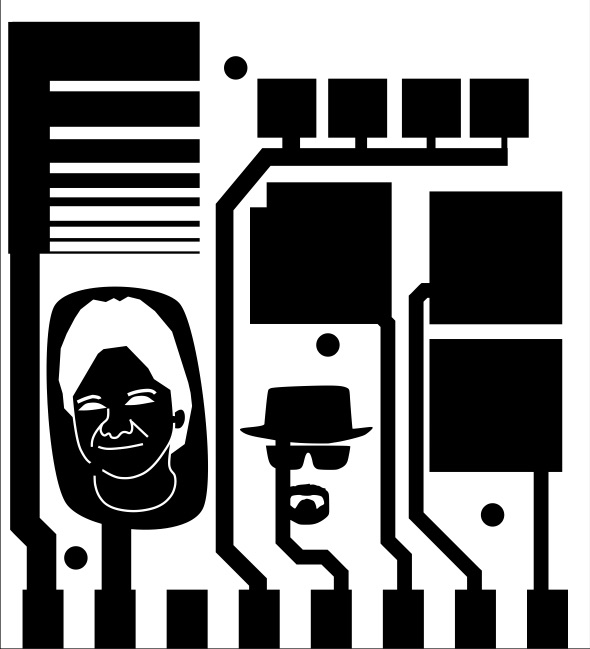
\includegraphics[width=0.2\textwidth, keepaspectratio]{./Bilder/testmuster-seite2.jpg}
  \label{testmuster-seite2}
  }
 \caption{Testmuster obere und untere Seite}
 \end{figure}

Qualitativ waren keine Unterschiede zu erkennen aber der Vorteil der Salzsäure liegt darin, dass sie die Ätzung schneller durchführt. Deshalb wir diese Methode gewählt.

\subsection{Oxidierung der Glasplatten}

%\textbf{Sicherheitshinweis:} Vorsicht beim Umgang mit den Chemikalien und immer eine Schutzbrille tragen.\\

Um die Oxidierung der Indium-Zinn Schicht der Glasplatten zu Indium-Zinn-Oxid zu erreichen wurden mehrere Verfahren getestet. Im Folgenden werden diese forgestellt und auf ihre Einsetzbarkeit überprüft.
Indikatoren für eine gelungene Oxidierung sind:
\begin{itemize}
\item Die für die leitende Schicht typische brauen Färbung muss merklich verschwinden
\item Eine Messung mittels eines Multimeters muss eine Nennenswerte Änderung der Leitfähigkeit ergeben\\
\end{itemize}

\subsubsection{Wasserstoffperoxid}

%\textbf{Sicherheitshinweis:} Vorsicht beim Umgang mit den Chemikalien und immer eine Schutzbrille tragen.\\

Eine Testplatte wurden in ein Wasserstoffperoxid-Bad gegeben und nach 1h wieder entnommen. Beide oben genannten Indikatoren haben nicht angesprochen, was darauf schließen lässt, dass der Oxidierungsversuch nicht erfolgreich war.
Nun soll ein Langzeittest über mehrere Tage Erkentnisse geben, ob der Oxidierungsvorgang bei einer längeren Einwirkungsdauer funktioniert. Dies war nicht der Fall.

Somit lässt sich festhalten, dass eine Oxidierung mittels Wasserstoffperoxid bei Raumtemperatur nicht möglich ist.\\

\subsubsection{Wasserstoffperoxid mit Hitze}

Da die Oxidierung bei Raumtemperatur nicht funktioniert hat wurde ein Versuch gestartet, die Indium-Zinn Schicht in erwärmten Wasserstoffperoxid durchzuführen.
Keiner der oben genannten Indikatoren wies auf eine Oxidierung hin, weshalb das Verfahren ebenfalls als nicht erfolgreich gewertet wird.\\

\subsubsection{Hitze durch einen Heißluftfön}

Ein Test mit einem Heißluftfön, der auf 300 Grad eingestellt wurde ergab, das nach einer Einwirkzeit von 1h die Schicht oxidiert ist. Jedoch ist keine großflächige Aufbringung der Hitze möglich. Deshalb ist für Plattengröße von 110mmx100mm das Verfahren unbrauchbar.\\

\subsubsection{Hitze im Ofen}

Ein funktionierendes, aber sehr zeitaufwändiges, Verfahren ist die Oxidierung in einem Ofen. Hierbei kann ein gewöhnlicher Pizzaofen eingesetzt werden. Wir haben den Reflow-Ofen aus dem Fablab hierfür benutzt.
Bei der maximalen Temperatur des Ofen von 230 Grad werden die Glasplatten mit der beschichteten Seite nach oben auf das Gitter gelegt. Wichtig ist, dass der Ofen maximal leicht vorgeheizt wurde, da zu starke Temperaturunterschiede die Glasplatten zum brechen bringen könnten. Nun wurden die Testplatten für 1:30h im Ofen belassen und anschließend für 30 min abgekühlt.
Beide Indikatoren haben angeschlagen was zeigt, dass die Oxidierung erfolgreich war.\\

Da dies das einzig funktionierende und effiziente Verfahren ist, wird es zur Herstellung der Displays eingesetzt.

\subsection{Ausrichtung der Glasplatten}

Die Glasplatten müssen exakt über einanderliegen, sodass sich die Anzeigesymbole perfekt gegenüberliegen. Denn nur wo sie sich exakt gegenüber liegen, wird eine scharfe Anzeige möglich sein.
Aus diesem Grund haben wir zuerst Punkte mit dem Folienplotter ausgeschnitten und vor dem Oxidationsvorgang auf den Glasplatten positioniert, denn zu diesem Zeitpunkt ist die braune leitende Schicht noch gut sichtbar. Allerdings schmelzen dies Punkte, wenn man die Glasplatten zur Oxidierung in den Ofen gibt, weshalb diese Methode nicht empfehlenswert ist.
Es hat sich herausgestellt, dass die Oxidierung im Ofen die leitende Struktur nicht komplett durchsichtig macht. Deshalb ist eine extra Aufbringung von Ausrichtungspunkten oder Ähnlichem nicht notwendig.\\
Die Platten können ohne Probleme anhand der schwachen braunen Restfäbrung ausgerichtet werden.

\subsection{Reinigung der Glasplatten}

%\textbf{Sicherheitshinweis:} Vorsicht beim Umgang mit den Chemikalien und immer eine Schutzbrille tragen.\\

Im nächsten Schritt müssen die Glasplatten gereinigt werden, da jede Verunreinigung dazu führen kann, dass ungewollte Flecken entstehen.
Das alkalische Reinigungsbad wird im Verhältnis 1:5 mit Wasser gemischt und anschließend in ein Gefäß gegeben, in das die Glasplatten hineingelegt werden können (siehe Bild f). Wenn man die Platten jeweils mit der leitende Seite nach Außen zeigend einlegt, können beide gleichzeitig gereinigt werden. Um einen Siedeverzug zu verhindern ist es notwendig, dass Siedesteinchen eingelegt werden. Nachdem die Glasplatten in das Gefäß gelegt wurden kann die Flüßigkeit mit einem Heizfeld zum kochen gebracht. Die Glasplatten für 5 min im kochenden Wasser belassen und dann erst wieder etwas abkühlen lassen. Die Glasplatten vorsichtig entnehmen, da große Temperaturunterschiede diese zum Springen bringen können.
Von nun an sollte darauf geachtet werden, dass die sauberen Platten nicht wieder durch Fussel oder Feuchtigkeit verunreinigt werden.

\subsection{Reiborientierung}

Jetzt müssen die leitenden Schichten noch einer Reiborientierung unterzogen werden. Hierzu die mit einem fusselfreien Tuch abgetrockneten Glasplatten mit der leitenden Seite nach oben auf eine rutschfeste und harte Unterlage legen. Jetzt mit einem fusselfreien Tuch mehrfach unter festem Druck in eine Richtung streichen (siehe Bild g). Glasplatte 1 muss genau um 90 Grad versetzt zur Glasplatte 2 orientiert werden.

\subsection{Verkleben und Befüllen}

Nun die zugeschnittene Abstandhalterfolie auf eine Glasplatte legen. Als Abstandhalterfolie kann die Folie einer gewöhnlichen Verpackung einer Zigarettenschatel verwendet werden. 
Anschließend die zweite Glasplatte auflegen und zur Ersten ausrichten, dass die Anzeigesymbole so exakt wie möglich übereinander liegen. Nun die zwei Glasplatten an den Abstandhalterfolien zusamendrücken und zwei gegenüberliegende Seiten mit 2-Komponentenkleber verkleben (siehe Bild H). Sobald dieser hart geworden ist kann mit der Befüllung des Flüssigkristalls begonnen werden.
Nur sehr wenig Flüssigkristall mit einer Pipette entnehmen und an eine offene Seite auftragen. Durch den Kapillareffekt zieht dieser von selbst ein (siehe Bild i). Wenn das Display komplett vom Flüssigkristall durchzogen ist können die beiden noch offenen Seiten ebenfalls mit 2-Komponentenkleber verklebt werden.\\

Wichtig ist, dass nicht an beiden Seiten der Flüssigkristall aufgetragen wird, sondern nur an Einer.
Die Abstandhalter in eine Richtung ausrichten, sodass kein Foliensterifen senkrecht zu einer anderen steht. Dadurch wird ein gutes einziehen des Flüsigkristalls gewährleistet. Querliegende Folienabschnitte verhindern einen zügigen und vollständigen Einzug.
Außerdem sollte darauf geachtet werden, dass die Folien am Rand angebracht werden. Würde die Folie in die Mitte gelegt kann an diese Stelle kein Flüssigkristall gelangen und somit enstehen Flecken an diesen Stellen (siehe Bild j).

\subsection{Anzeigefähigkeit}
Selbst die kleinste Zuleitung (Dicke 1mm) bei den kleinen Rechtecken versorgt diese sicher mit Spannung und sie können somit angezeigt werden. Die kleinste Struktur beim Strukturtest wird ohne Probleme angezeigt (Dicke 0,4mm). Der Grund dafür sind die scharfen Kanten, die durch den Folienplott erreicht werden. Die Ausrichtung ist gut möglich, da die Struktur nach der Oxidierung der Glasplatten noch leicht, aber dennoch gut sichtbar ist. Komplexe Strukturen (Walter White, Darth Vader, Jürgen) können ebenso ohne Probleme angezeigt werden.

\begin{figure}[]
    \centering
    %\subfigure[Caption]{   
       % 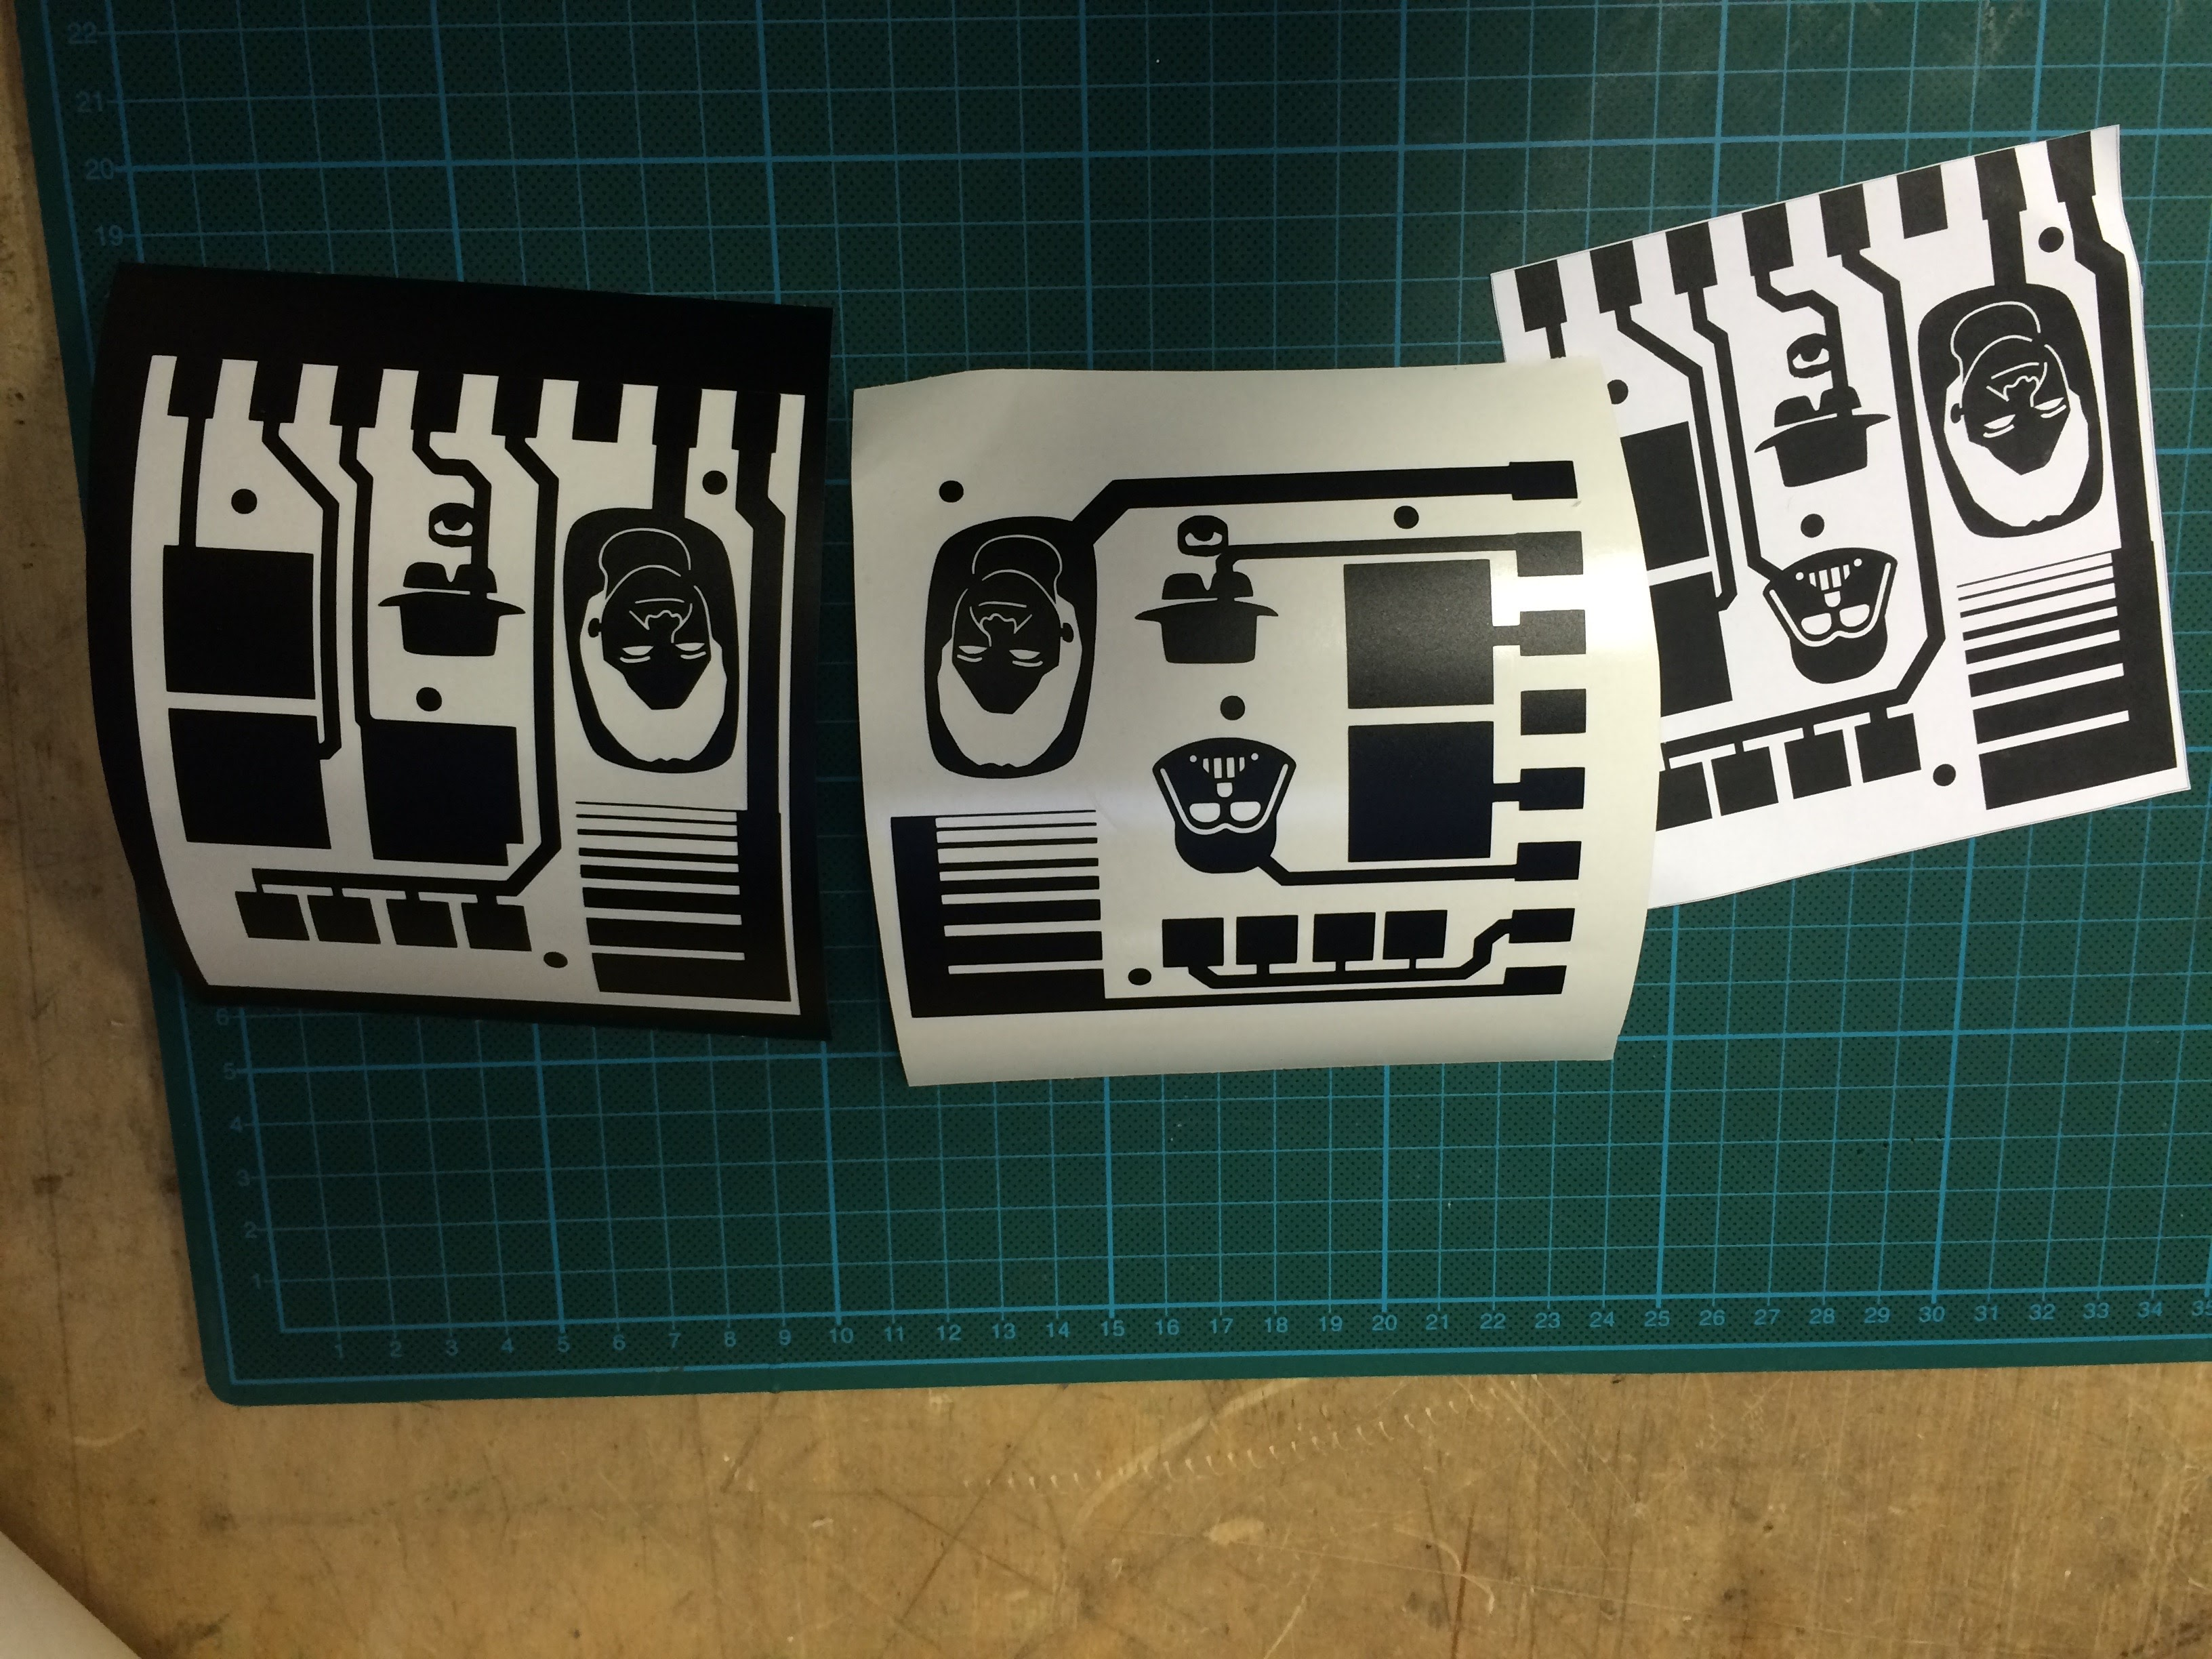
\includegraphics[width=0.22\textwidth]{./Bilder/Folie.jpg}
    %}
    %~ 
    \subfigure[Übertragen der Klebefolie]{  
        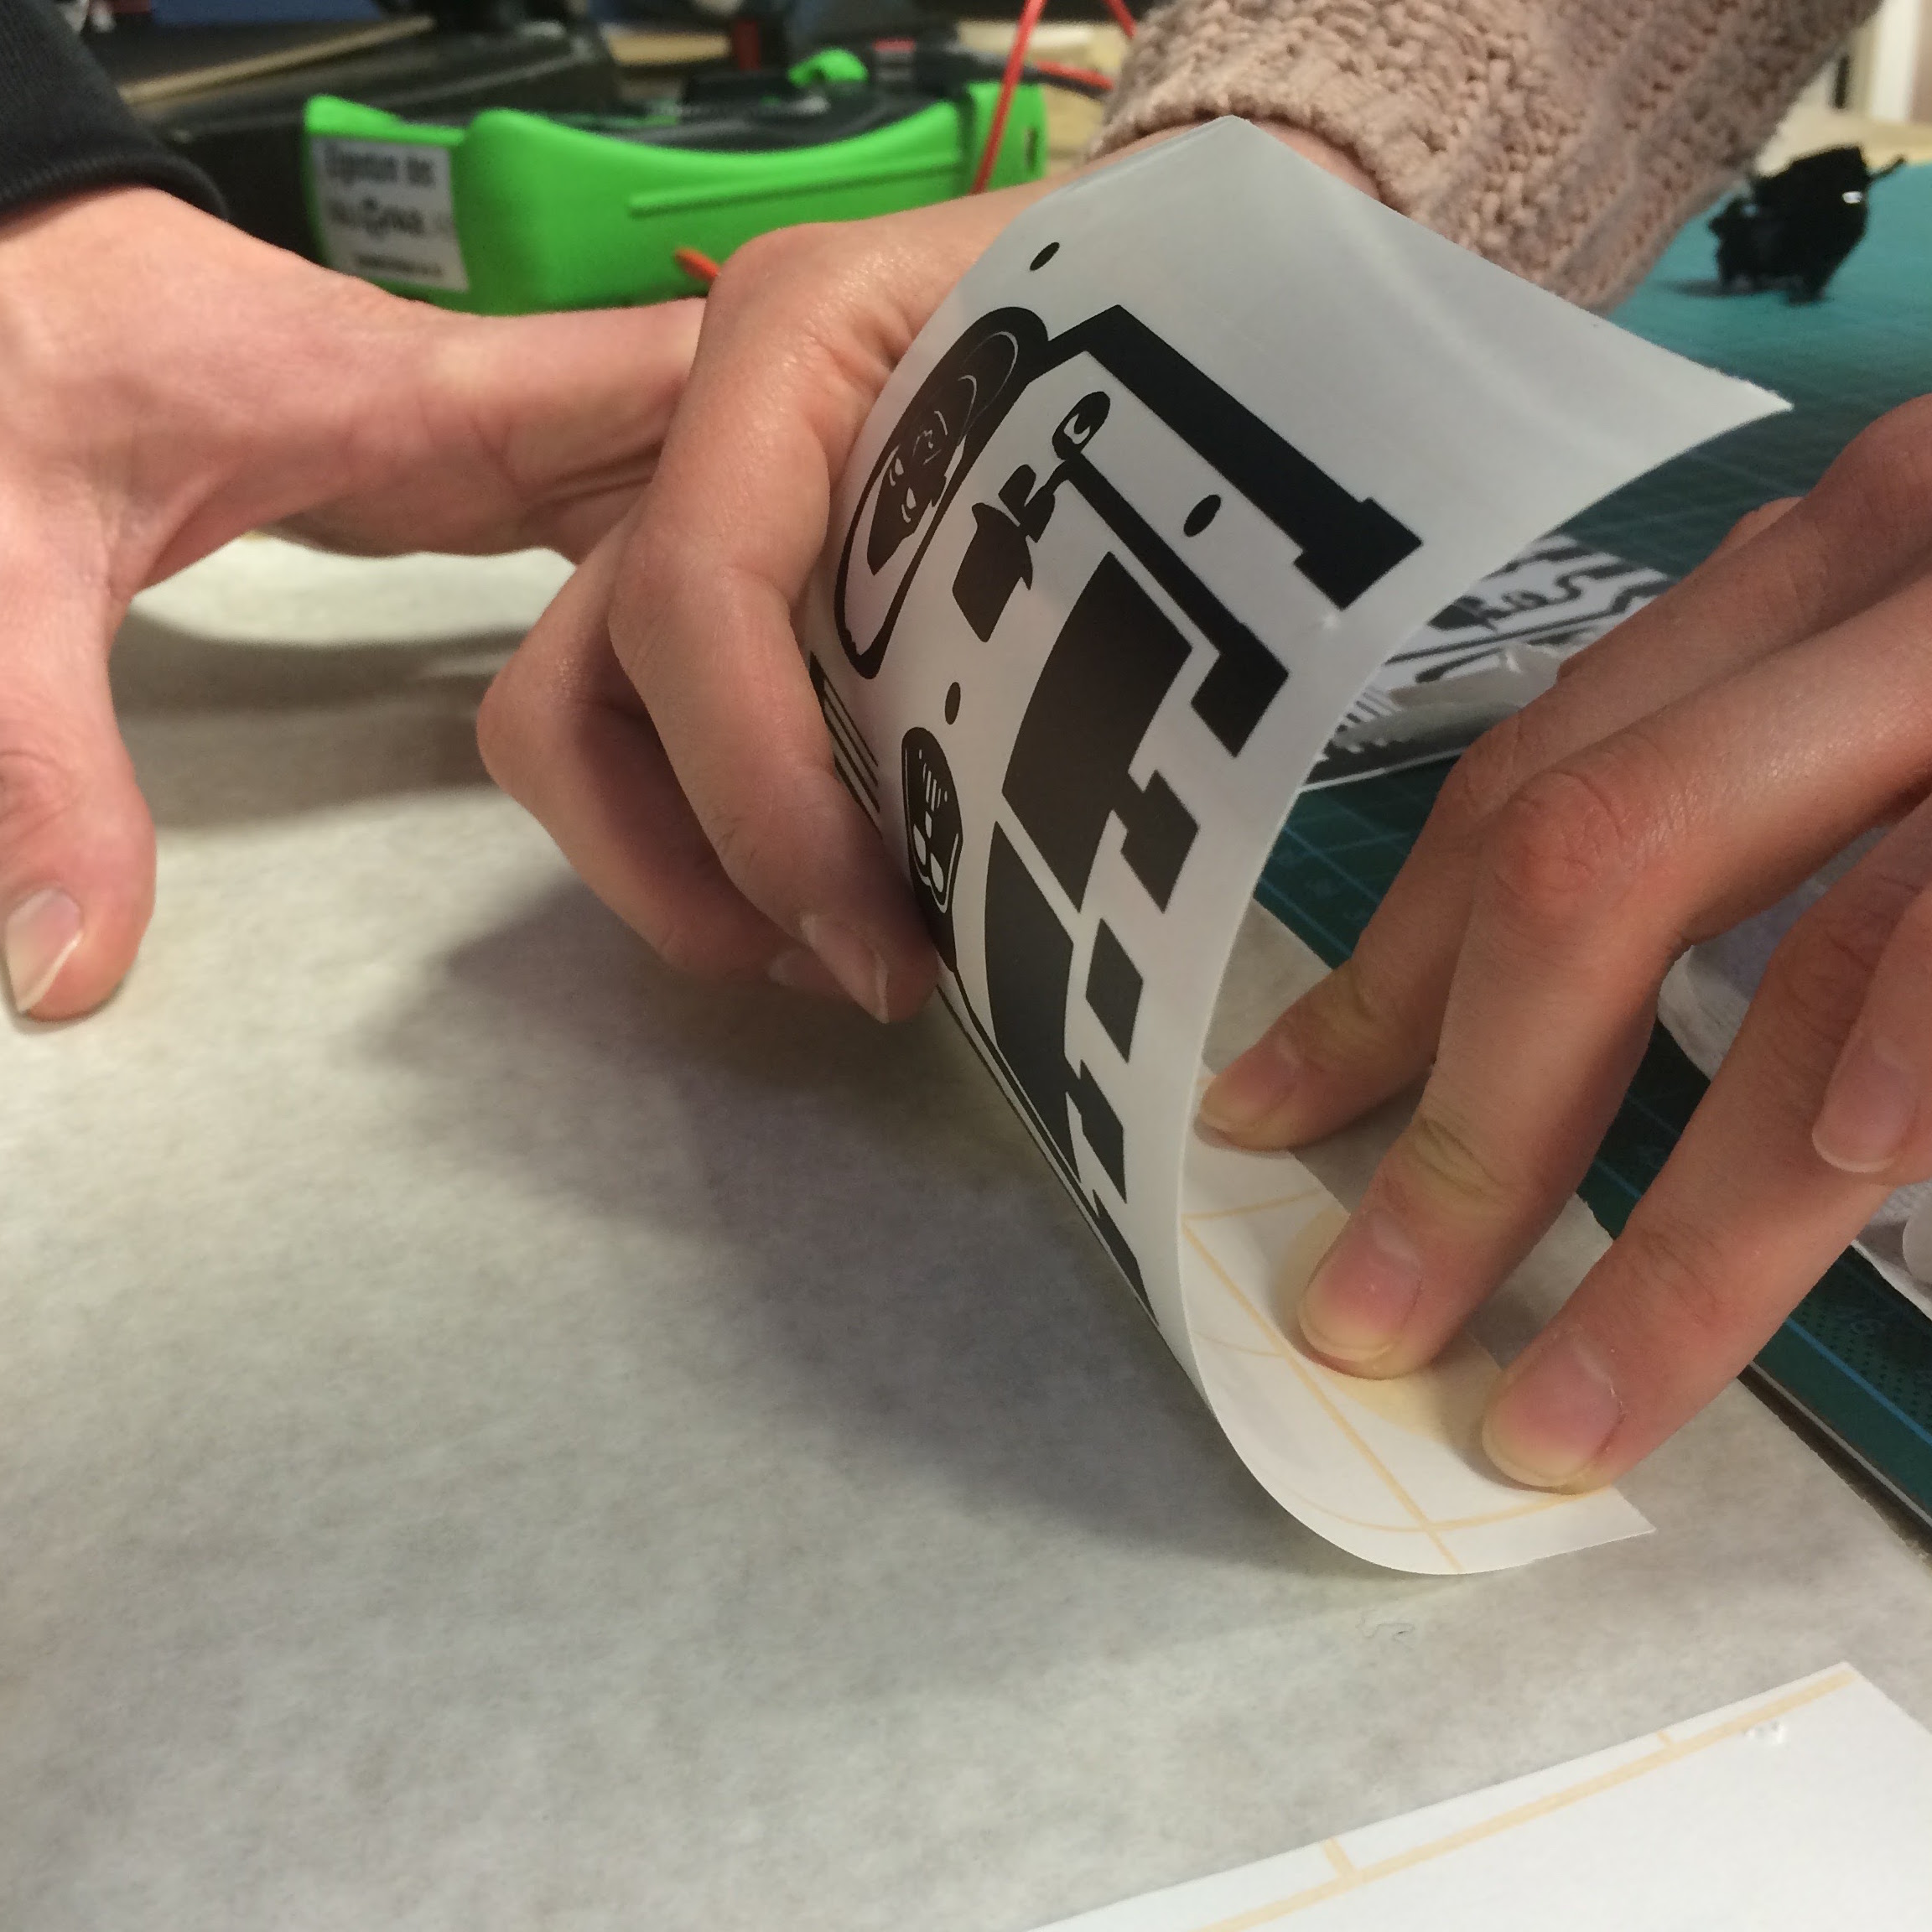
\includegraphics[width=0.22\textwidth]{./Bilder/aufklebenDerFolie.jpg}    
    }
    ~
     \subfigure[Ätzvorgang]{
   		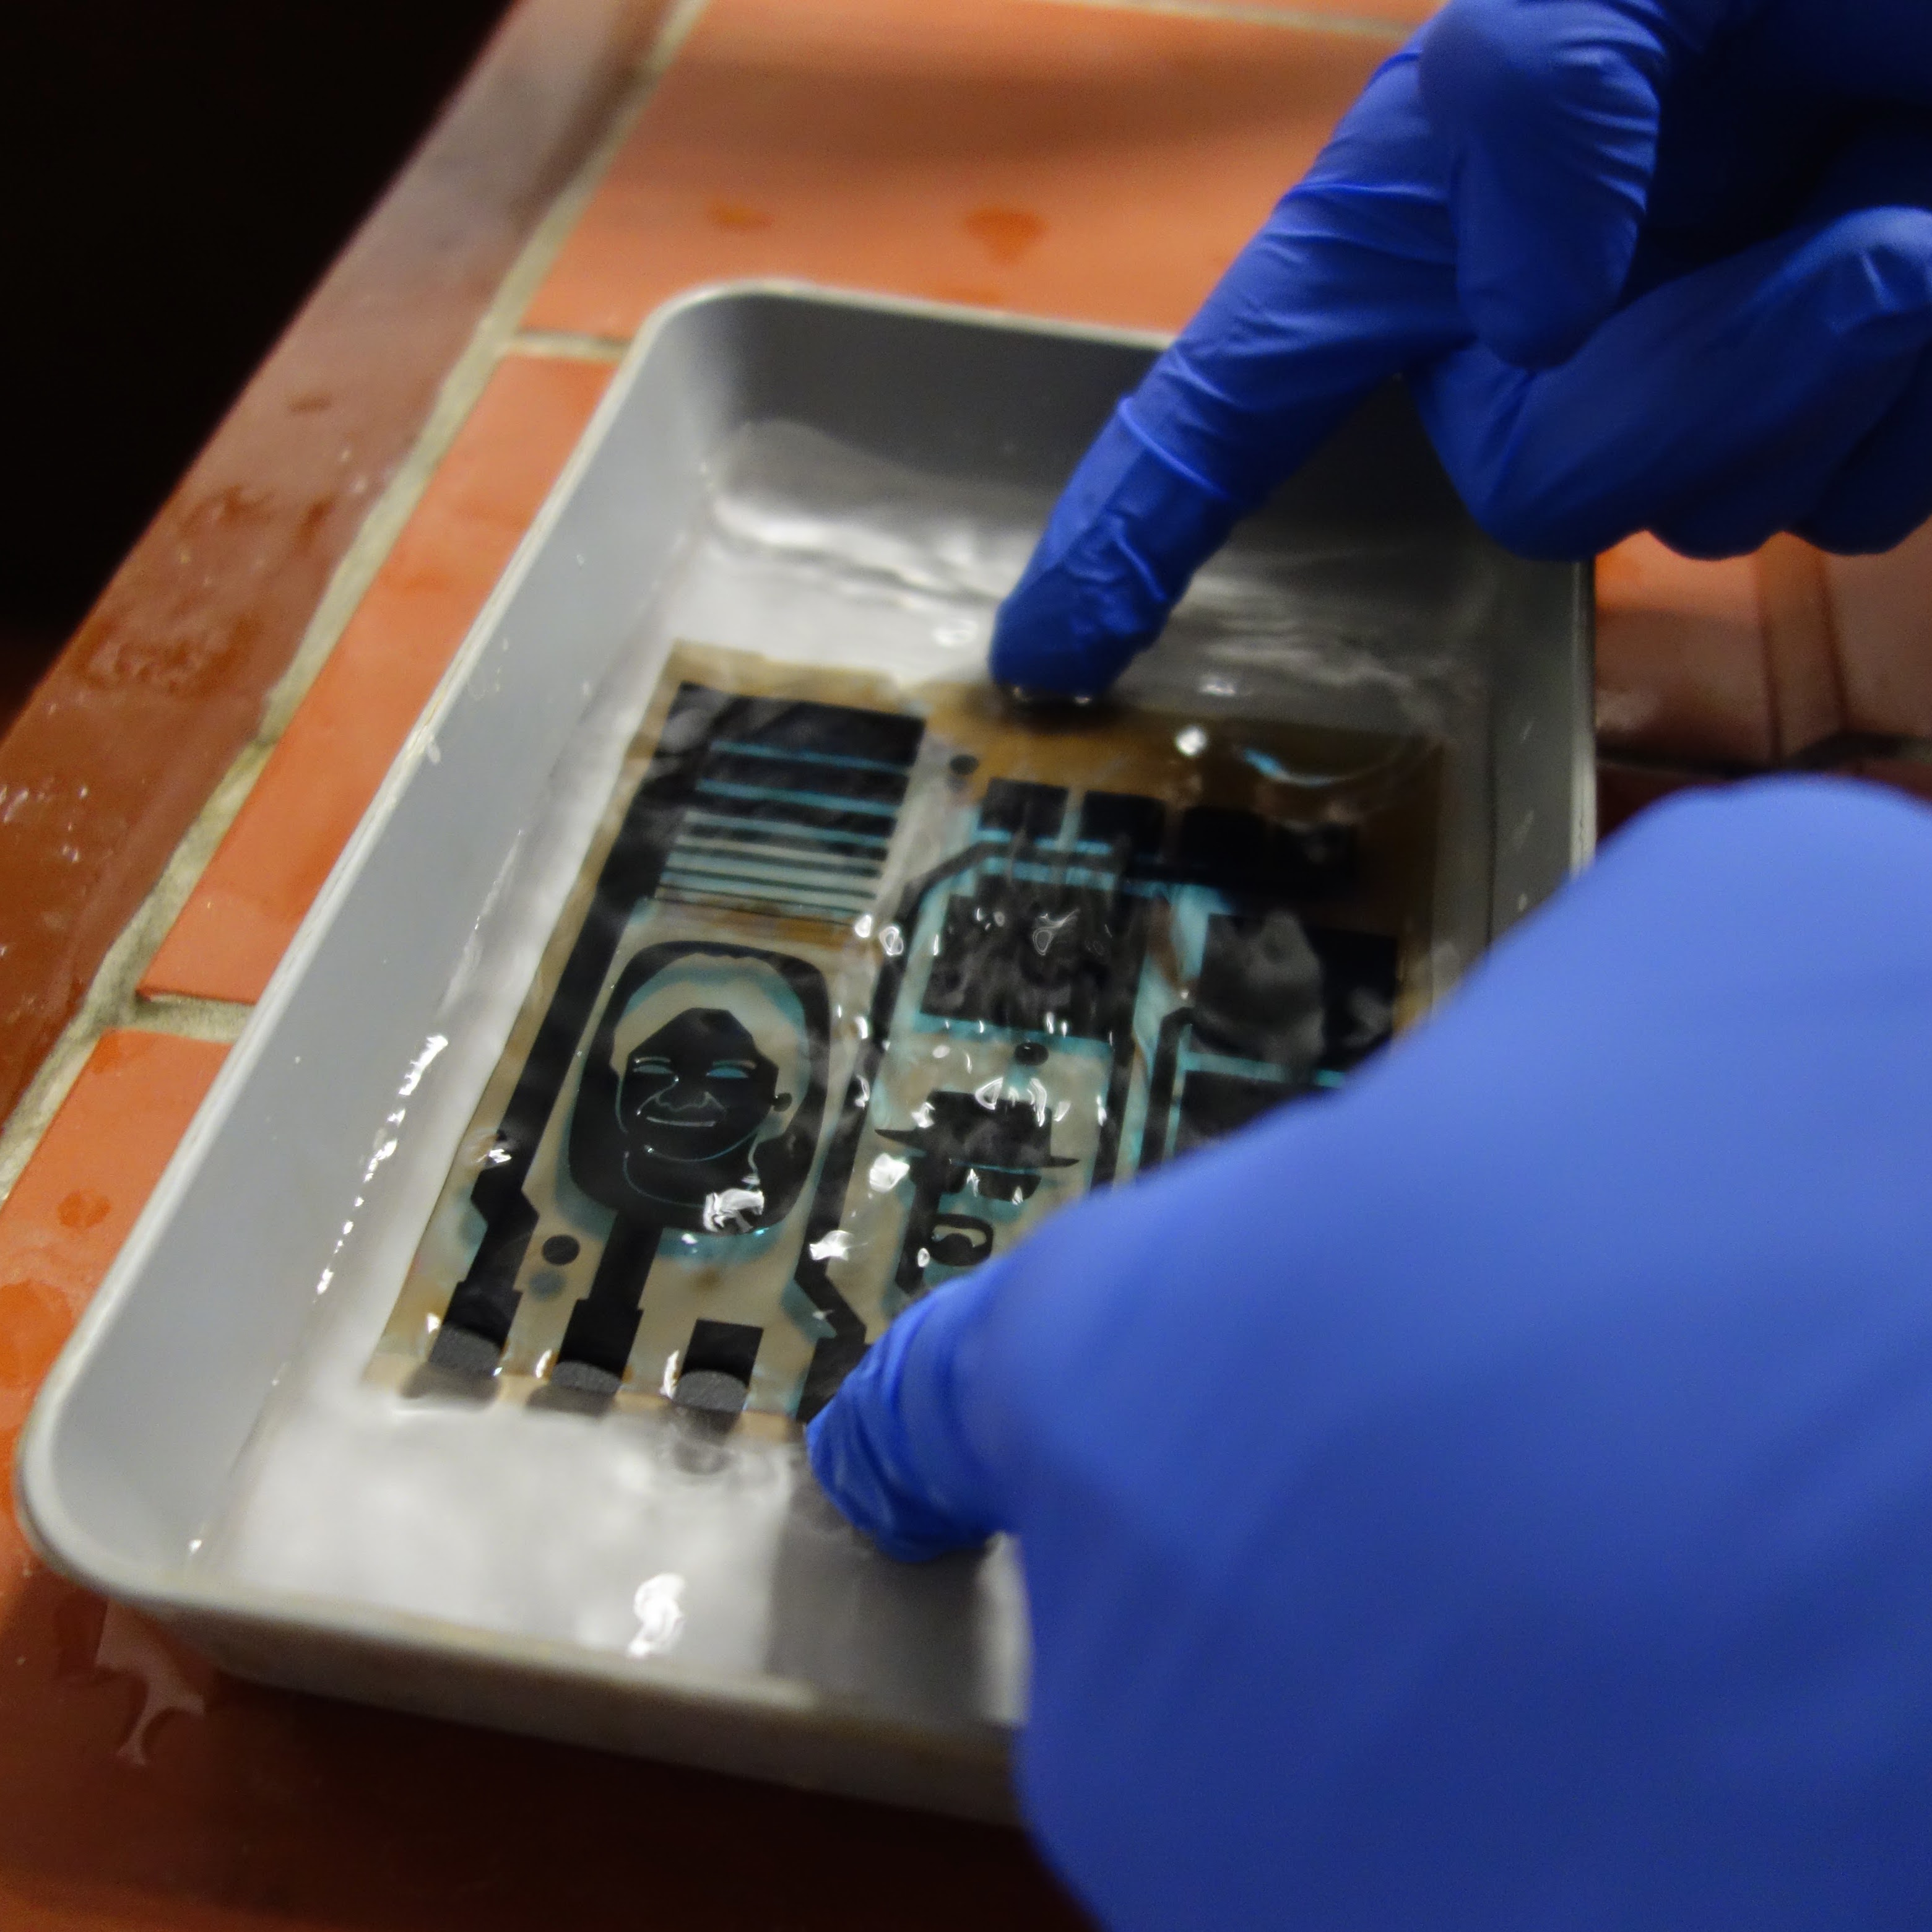
\includegraphics[width=0.22\textwidth]{./Bilder/aetzen.jpg}
    }
    ~
     \subfigure[Glasscheibe nach Ätzvorgang]{
   		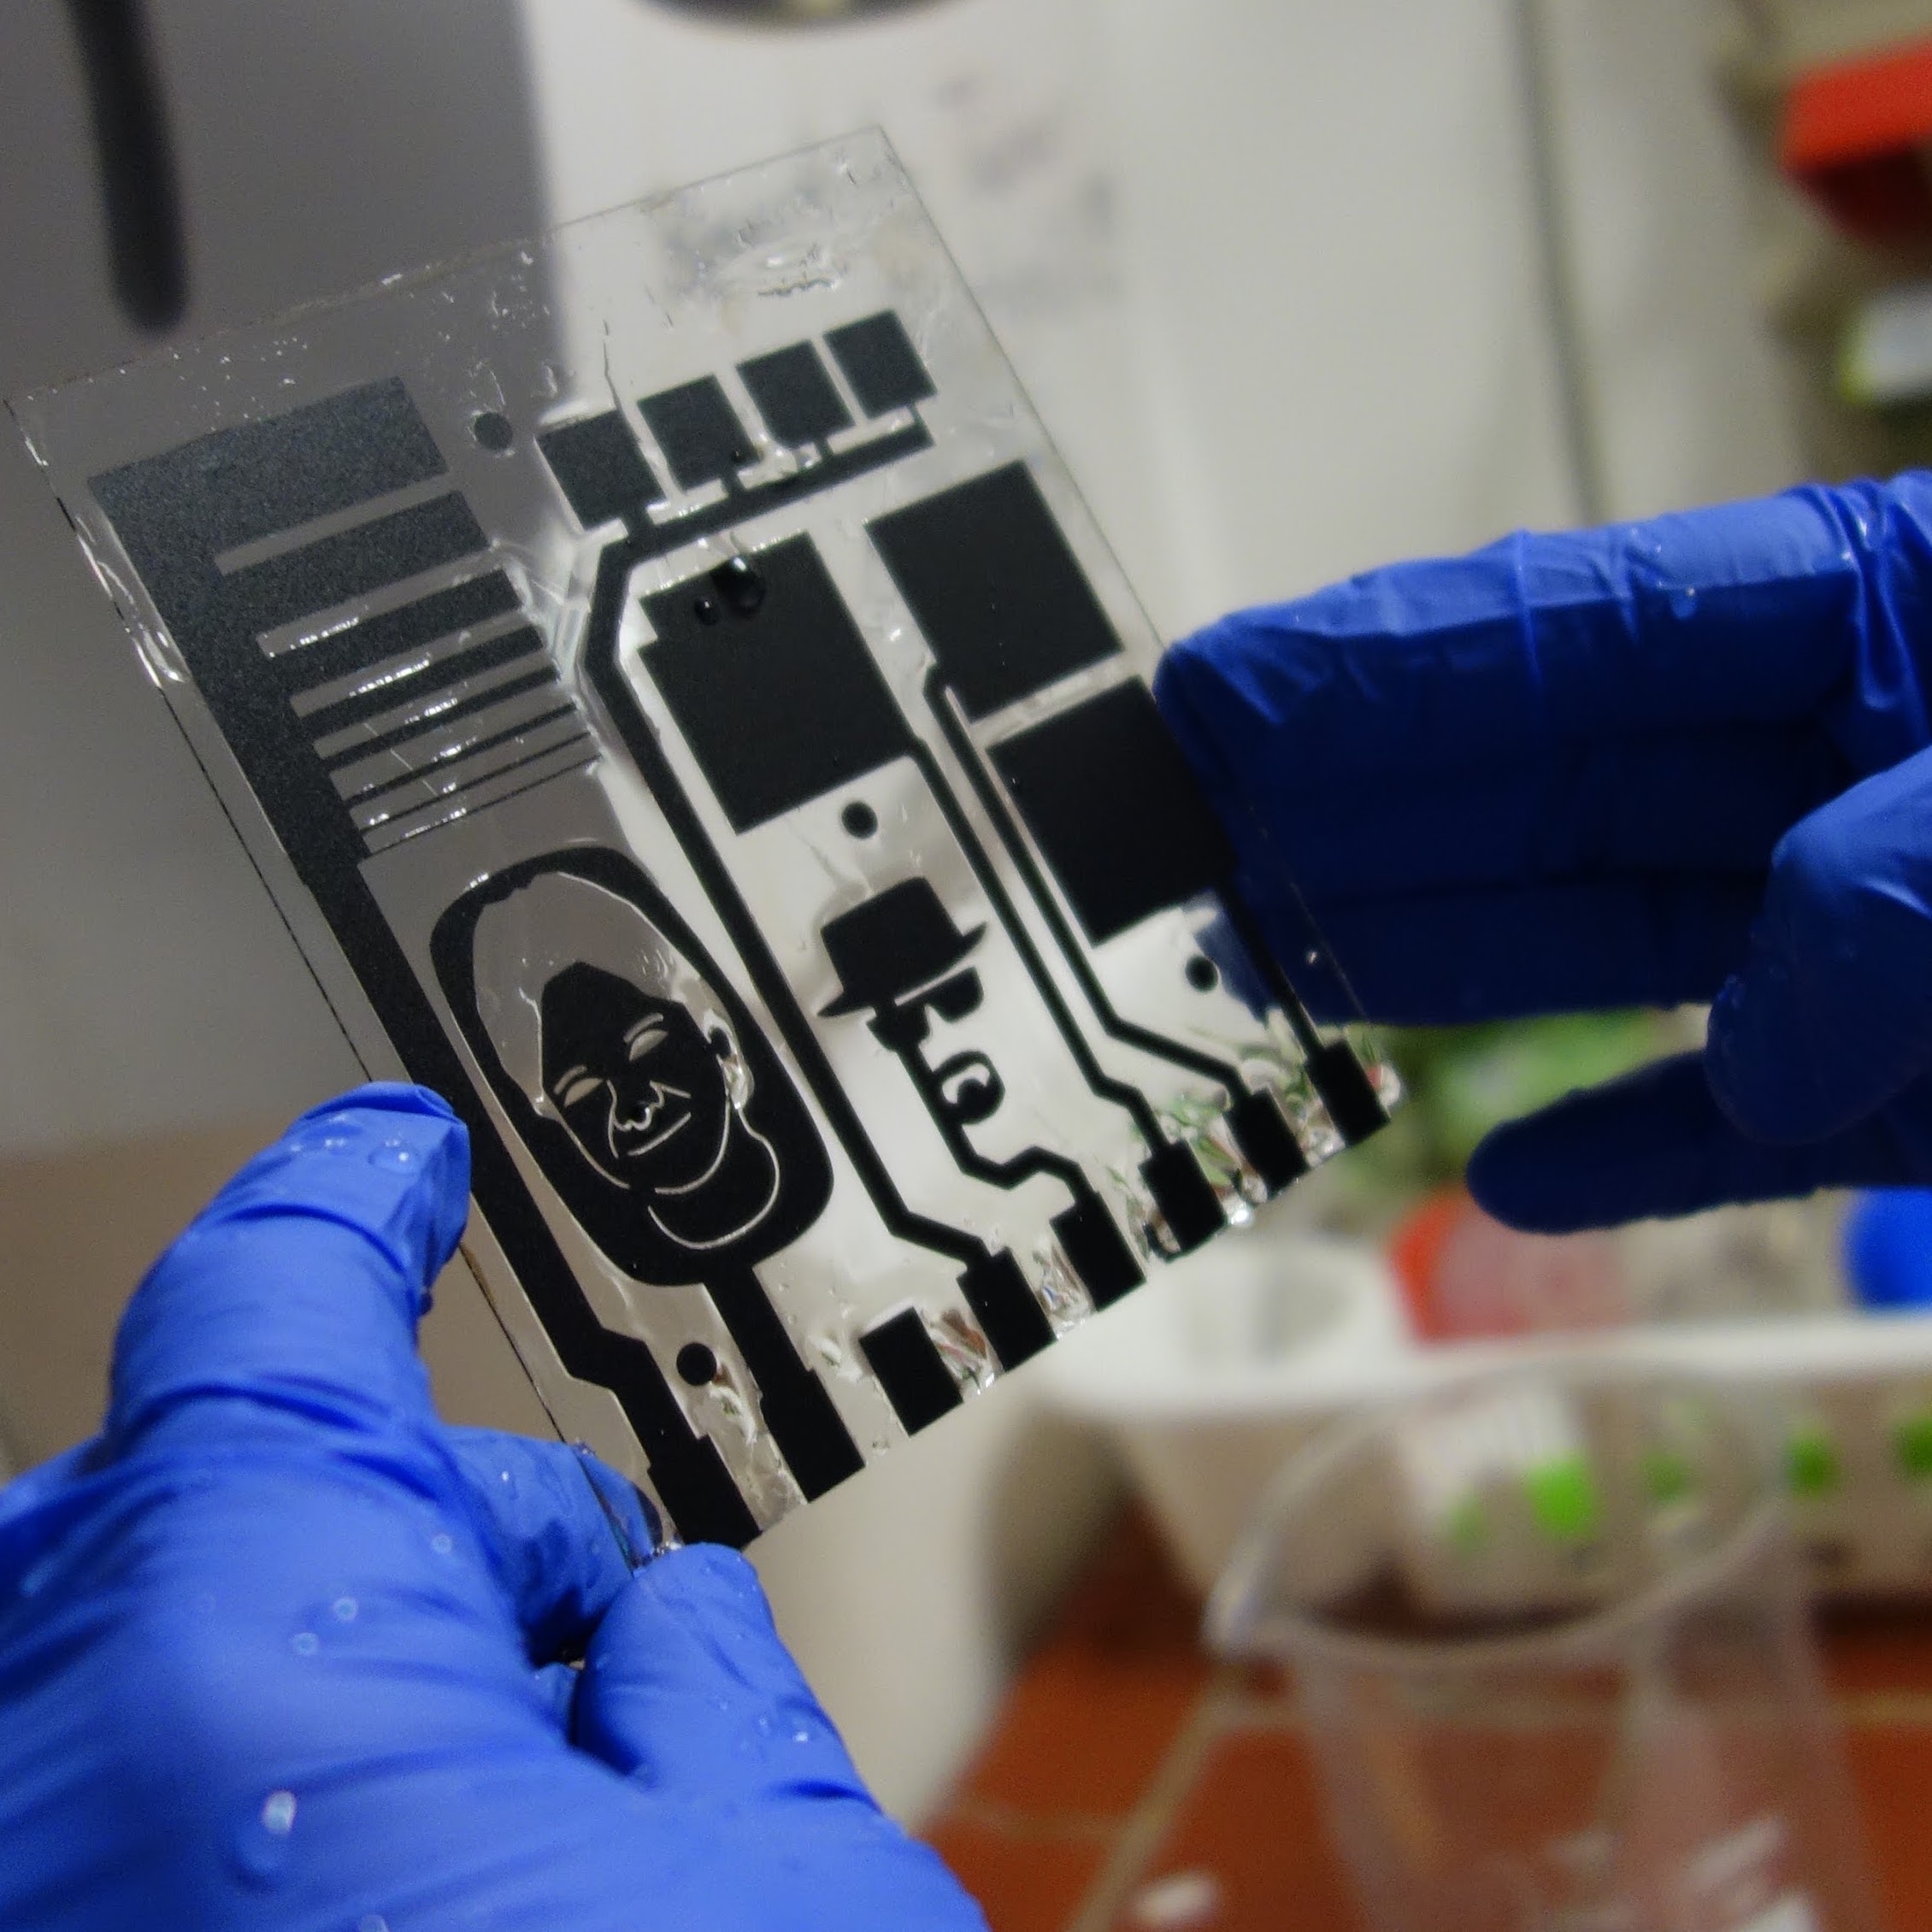
\includegraphics[width=0.22\textwidth]{./Bilder/Schritt3.jpg}
    }
    ~
    \subfigure[Abziehen der Folie]{	
   		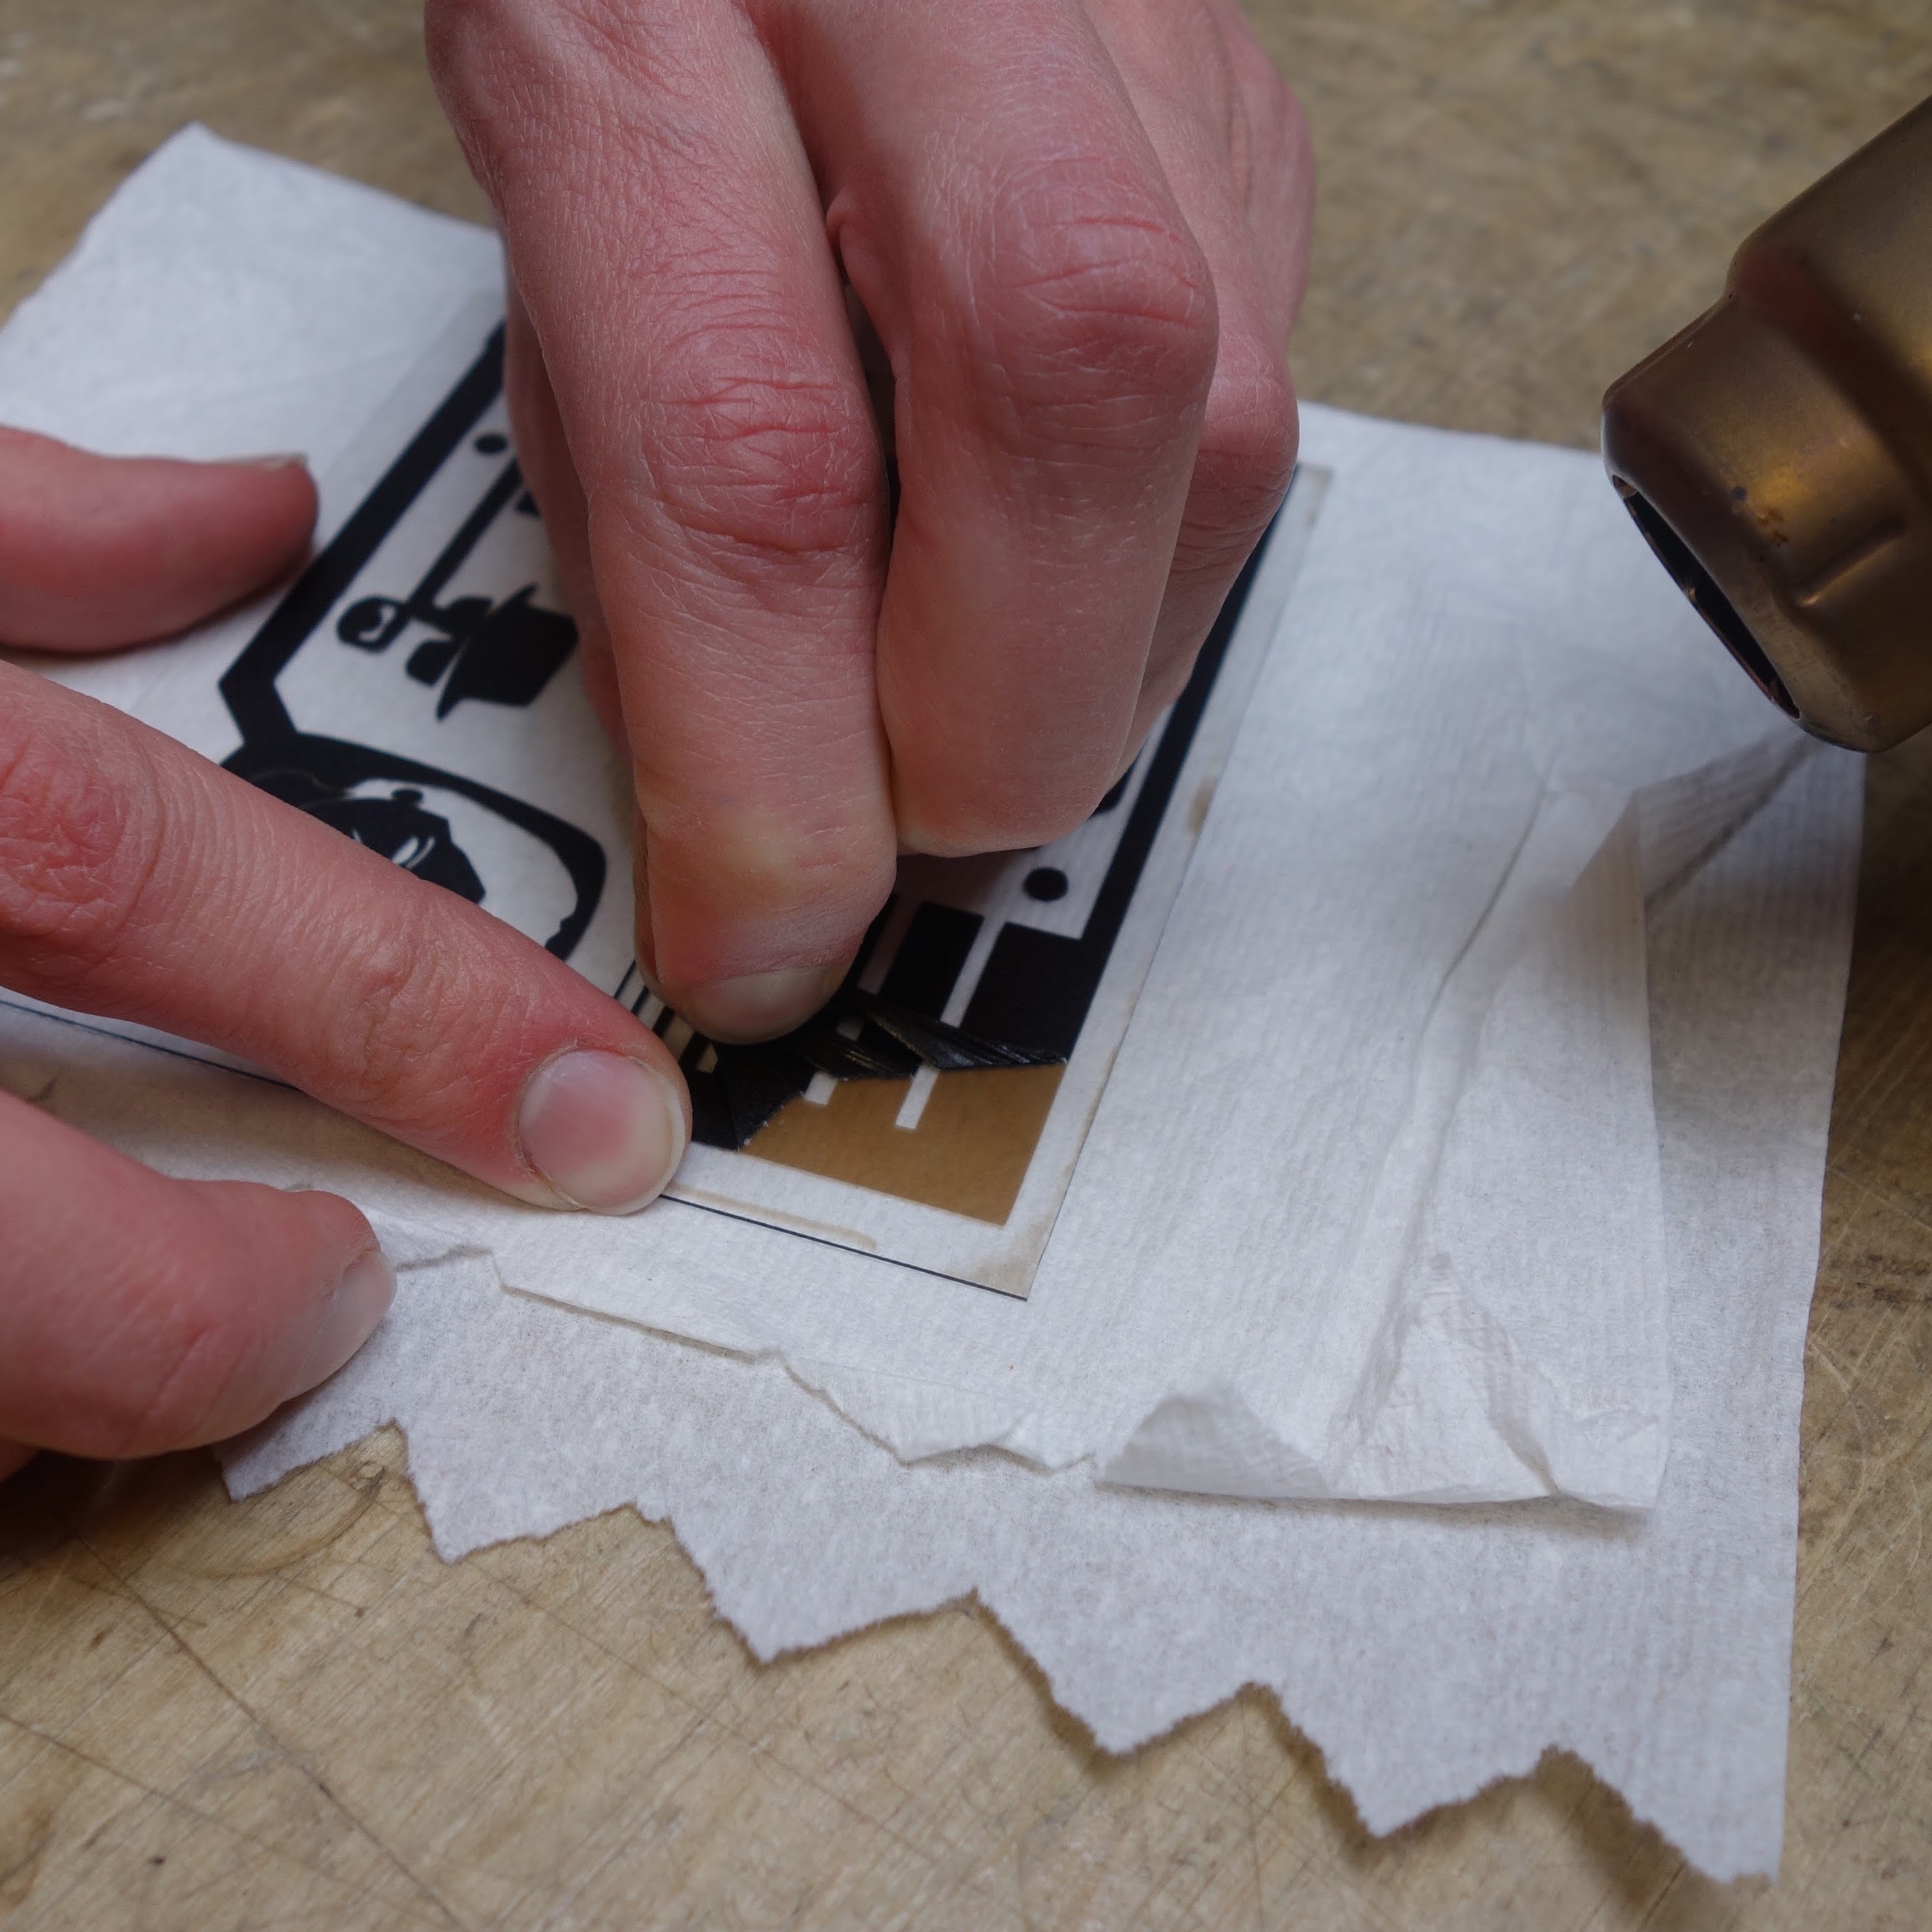
\includegraphics[width=0.22\textwidth]{./Bilder/Schritt2.jpg}
    }
    ~
    \subfigure[Oxidieren der Glasplatten]{	
   		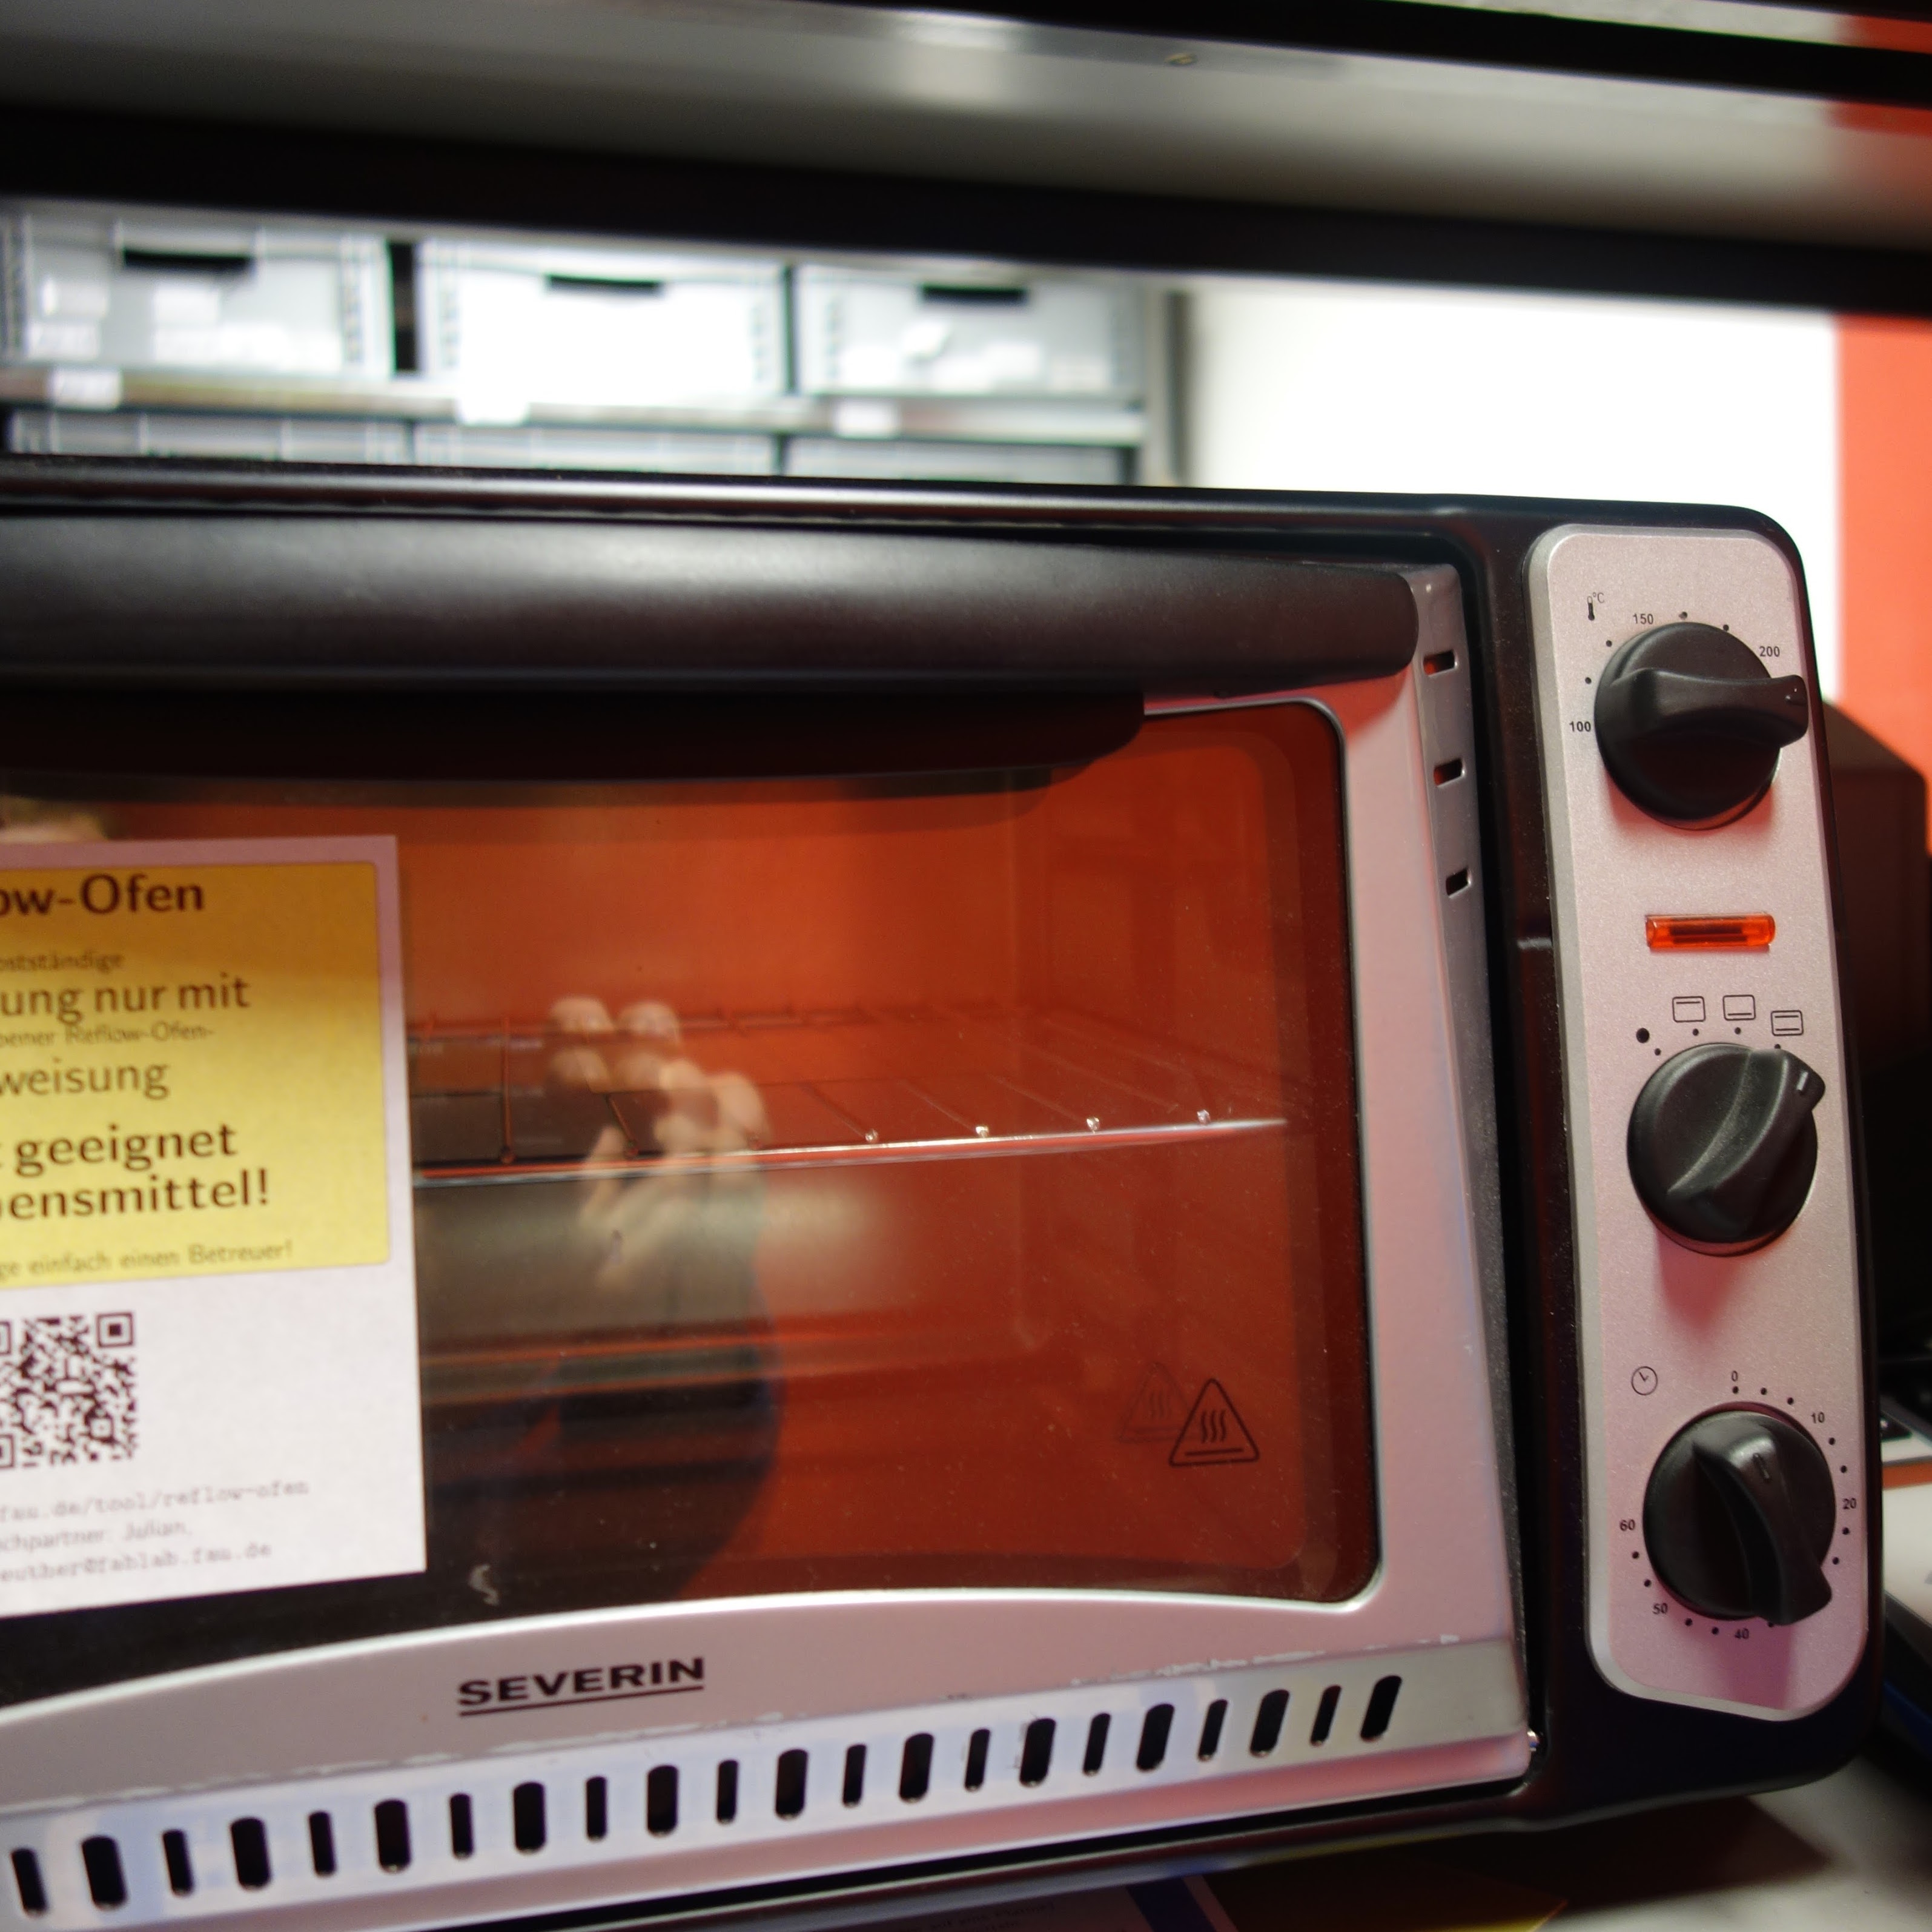
\includegraphics[width=0.22\textwidth]{./Bilder/backenImOfen.jpg}
    }
     ~
    \subfigure[Reinigen der Platten]{	
   		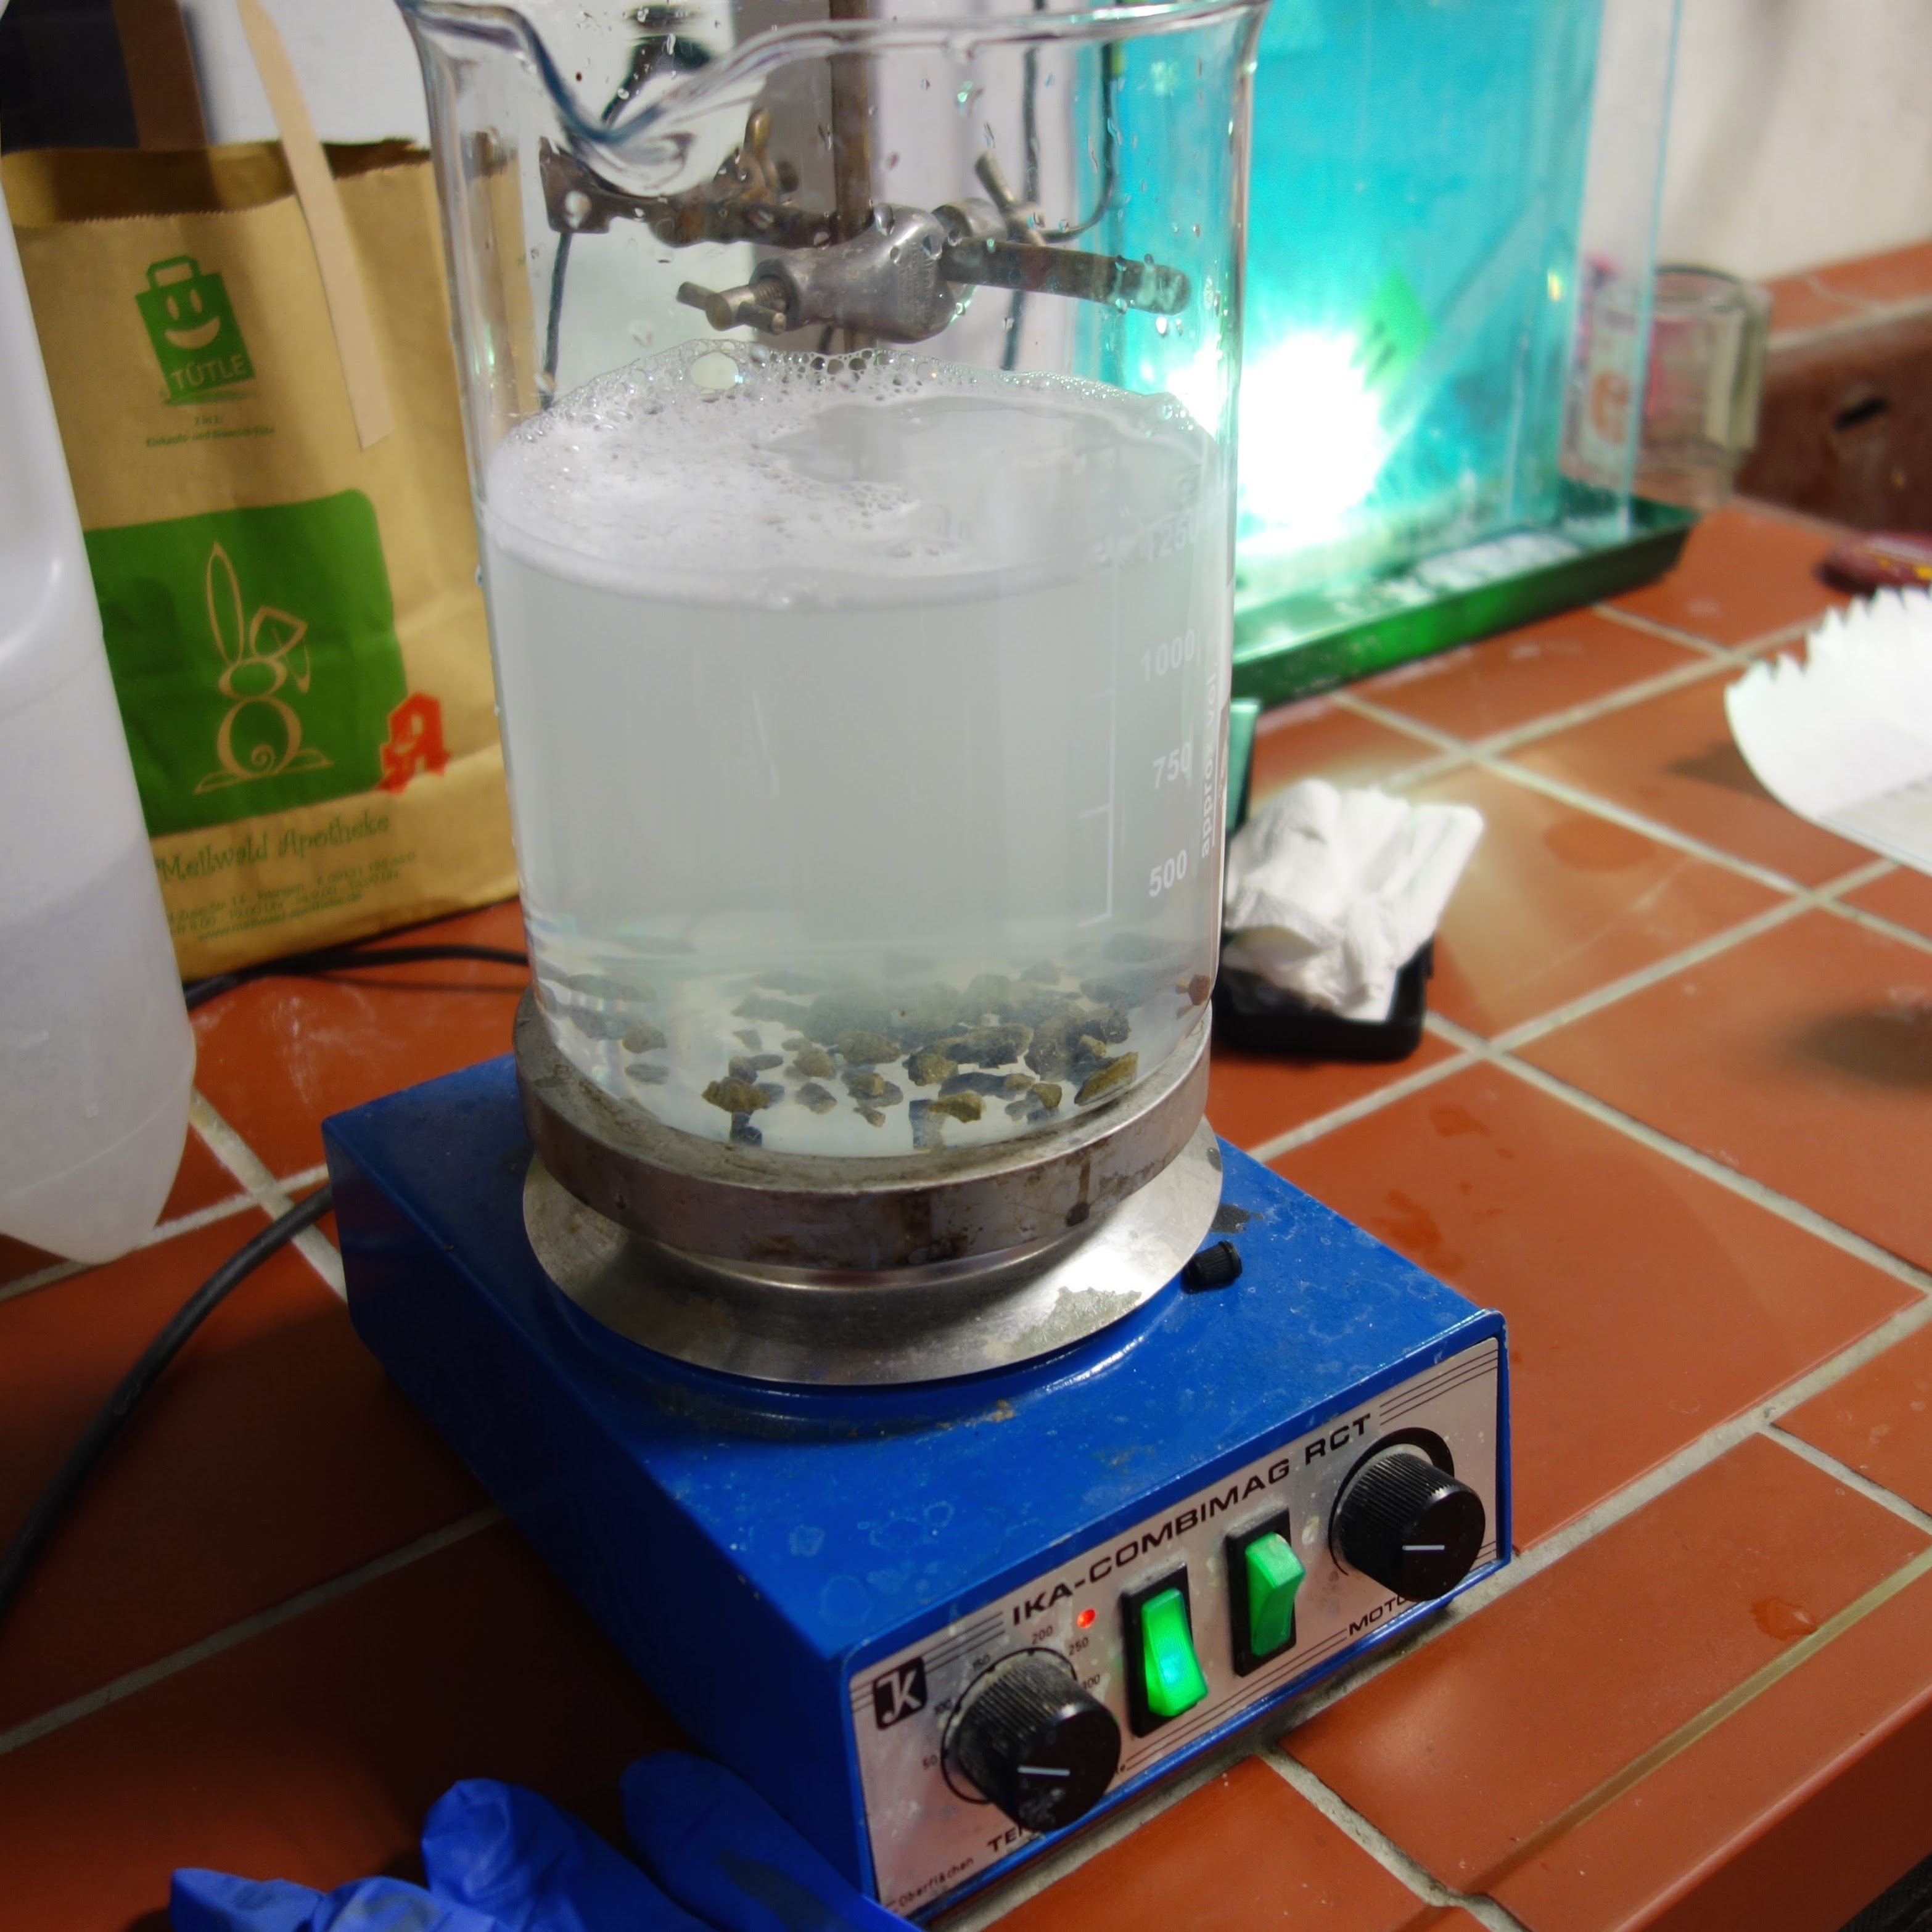
\includegraphics[width=0.22\textwidth]{./Bilder/cleanenDerPlatten.jpg}
    }
    ~
      \subfigure[Orientierung der Moleküle durch Reiben]{
   		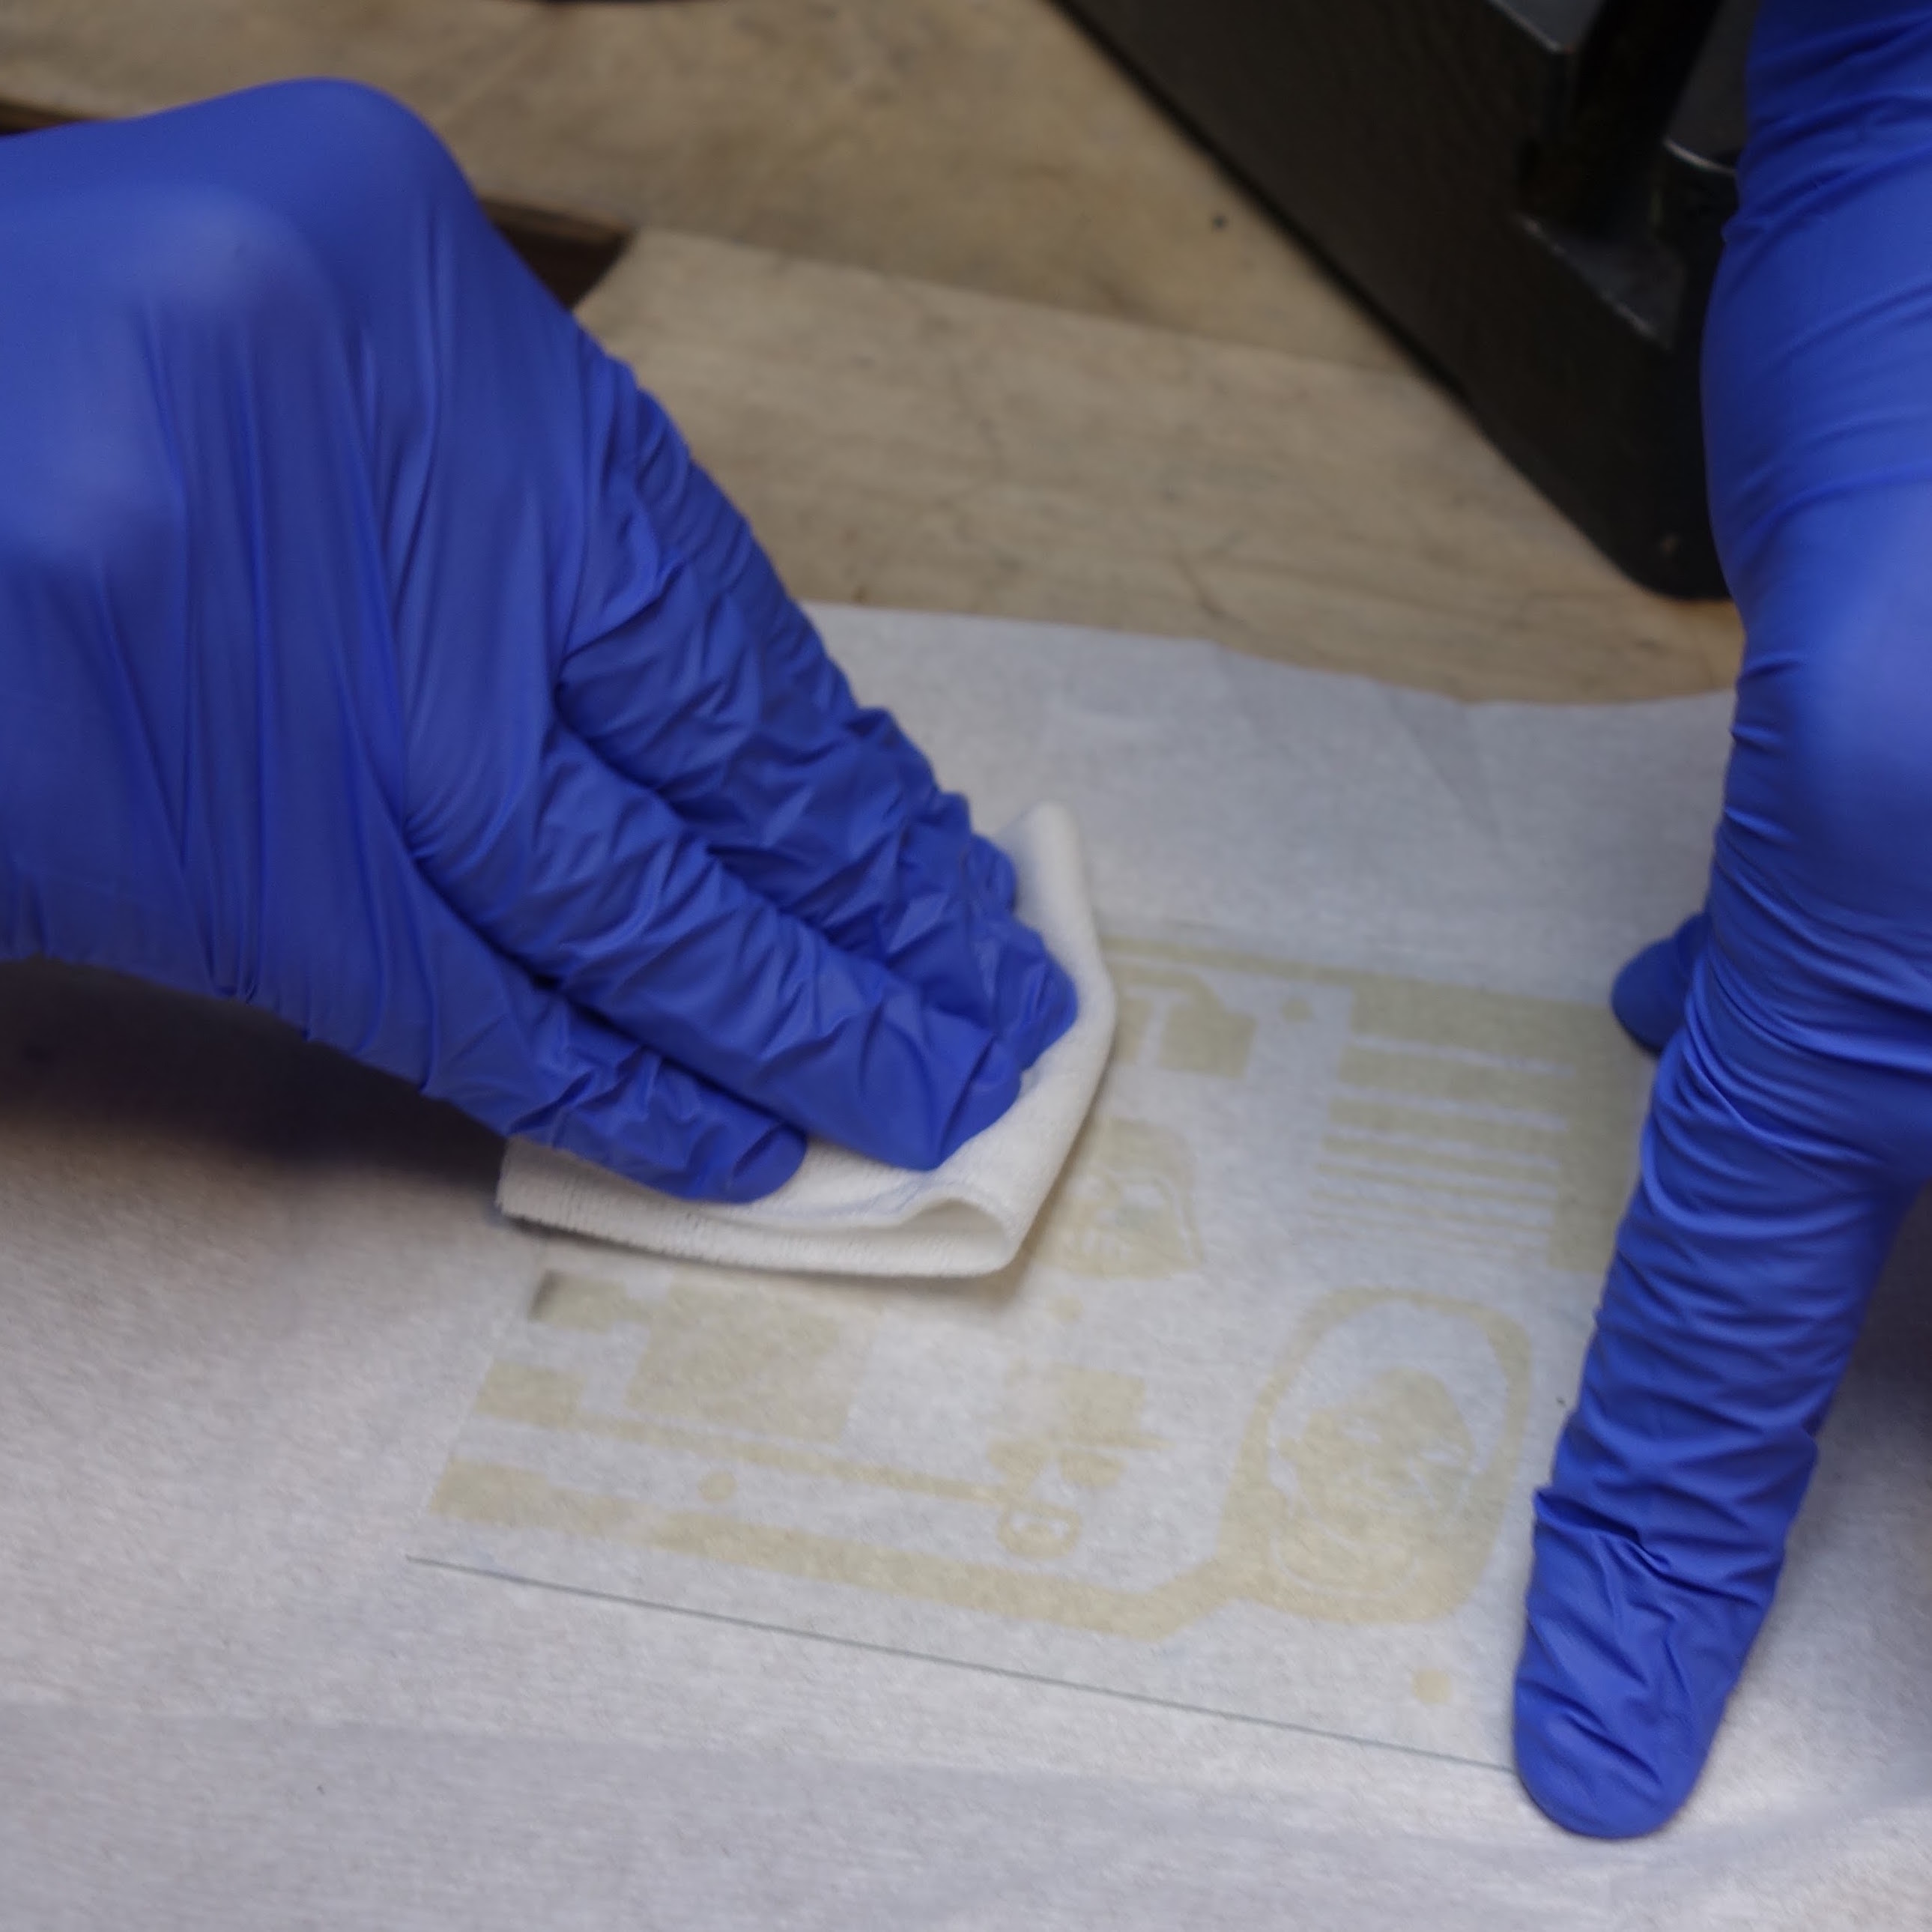
\includegraphics[width=0.22\textwidth]{./Bilder/Reiborientierung.jpg}
    }
    ~
      \subfigure[Verkleben von zwei Seiten des Displays]{
   		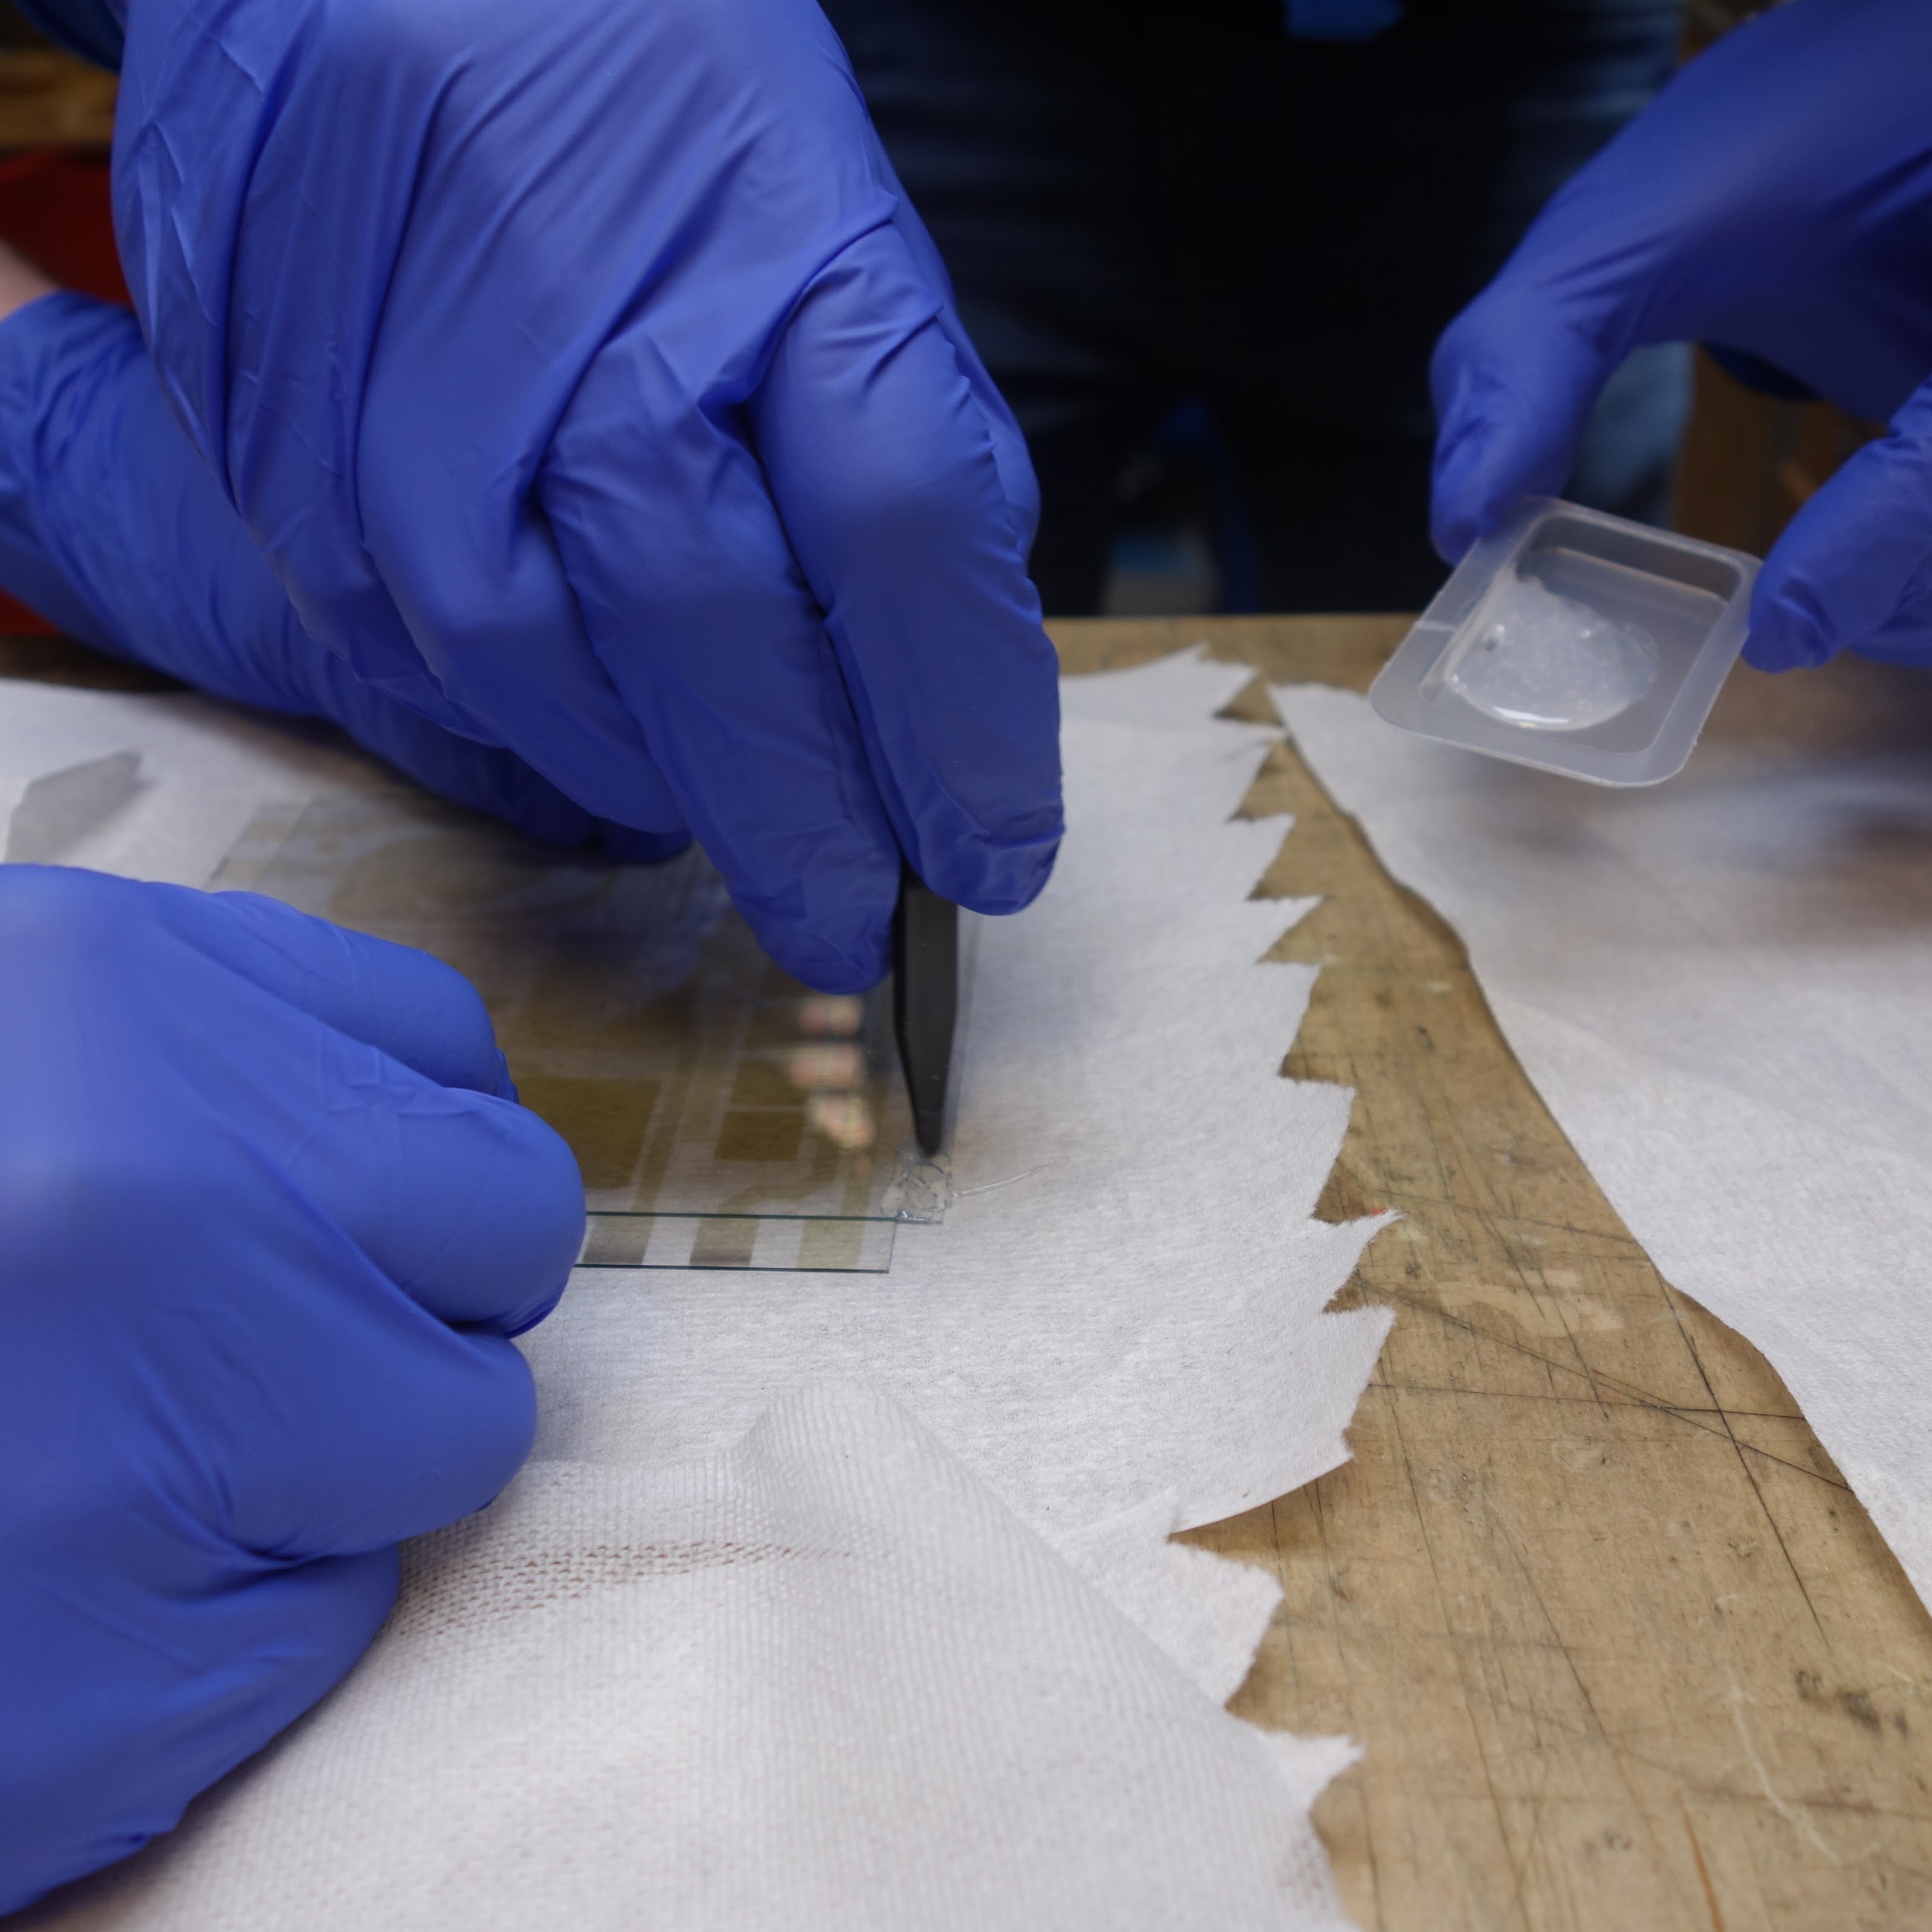
\includegraphics[width=0.22\textwidth]{./Bilder/verklebenDerPlatten.jpg}
    }
    ~
      \subfigure[Einführen des Flüssigkristalls und Verkleben der restlichen Seiten]{
   		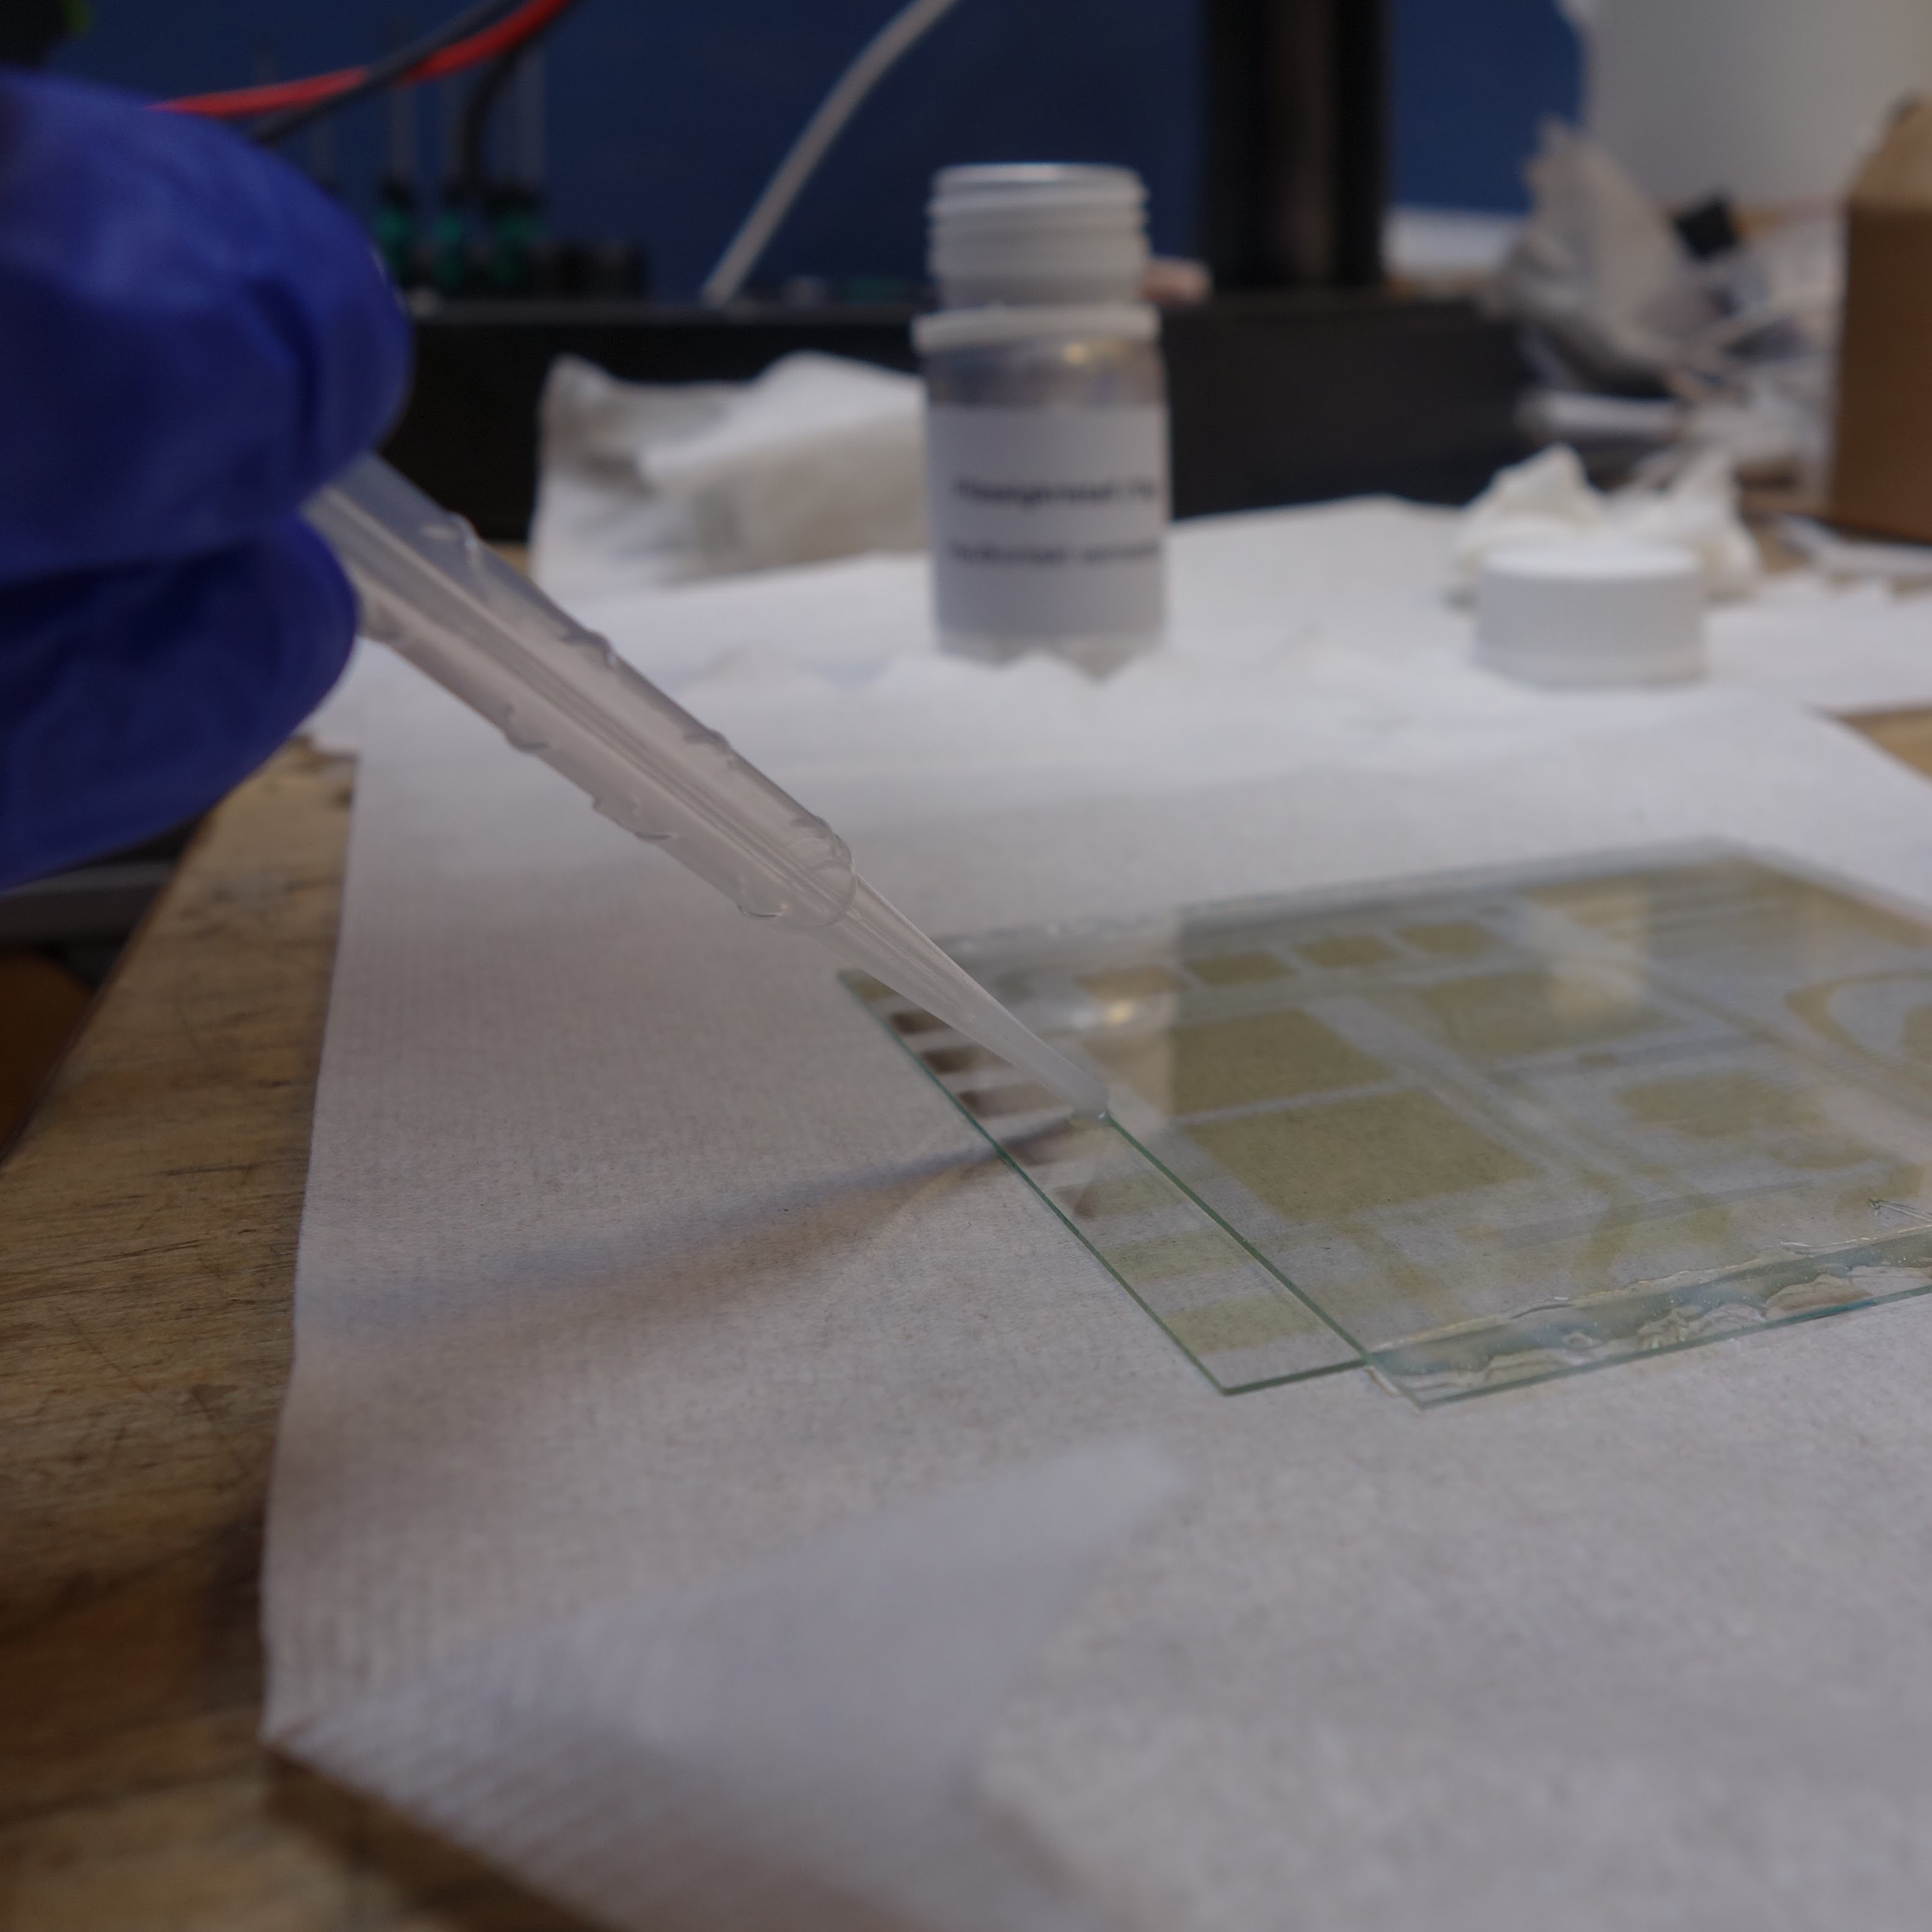
\includegraphics[width=0.22\textwidth]{./Bilder/liquidCeinfuegen.jpg}
    }
    ~
    \subfigure[Anbringen von Polarisationsfolien und Anlegen von Spannung]{
		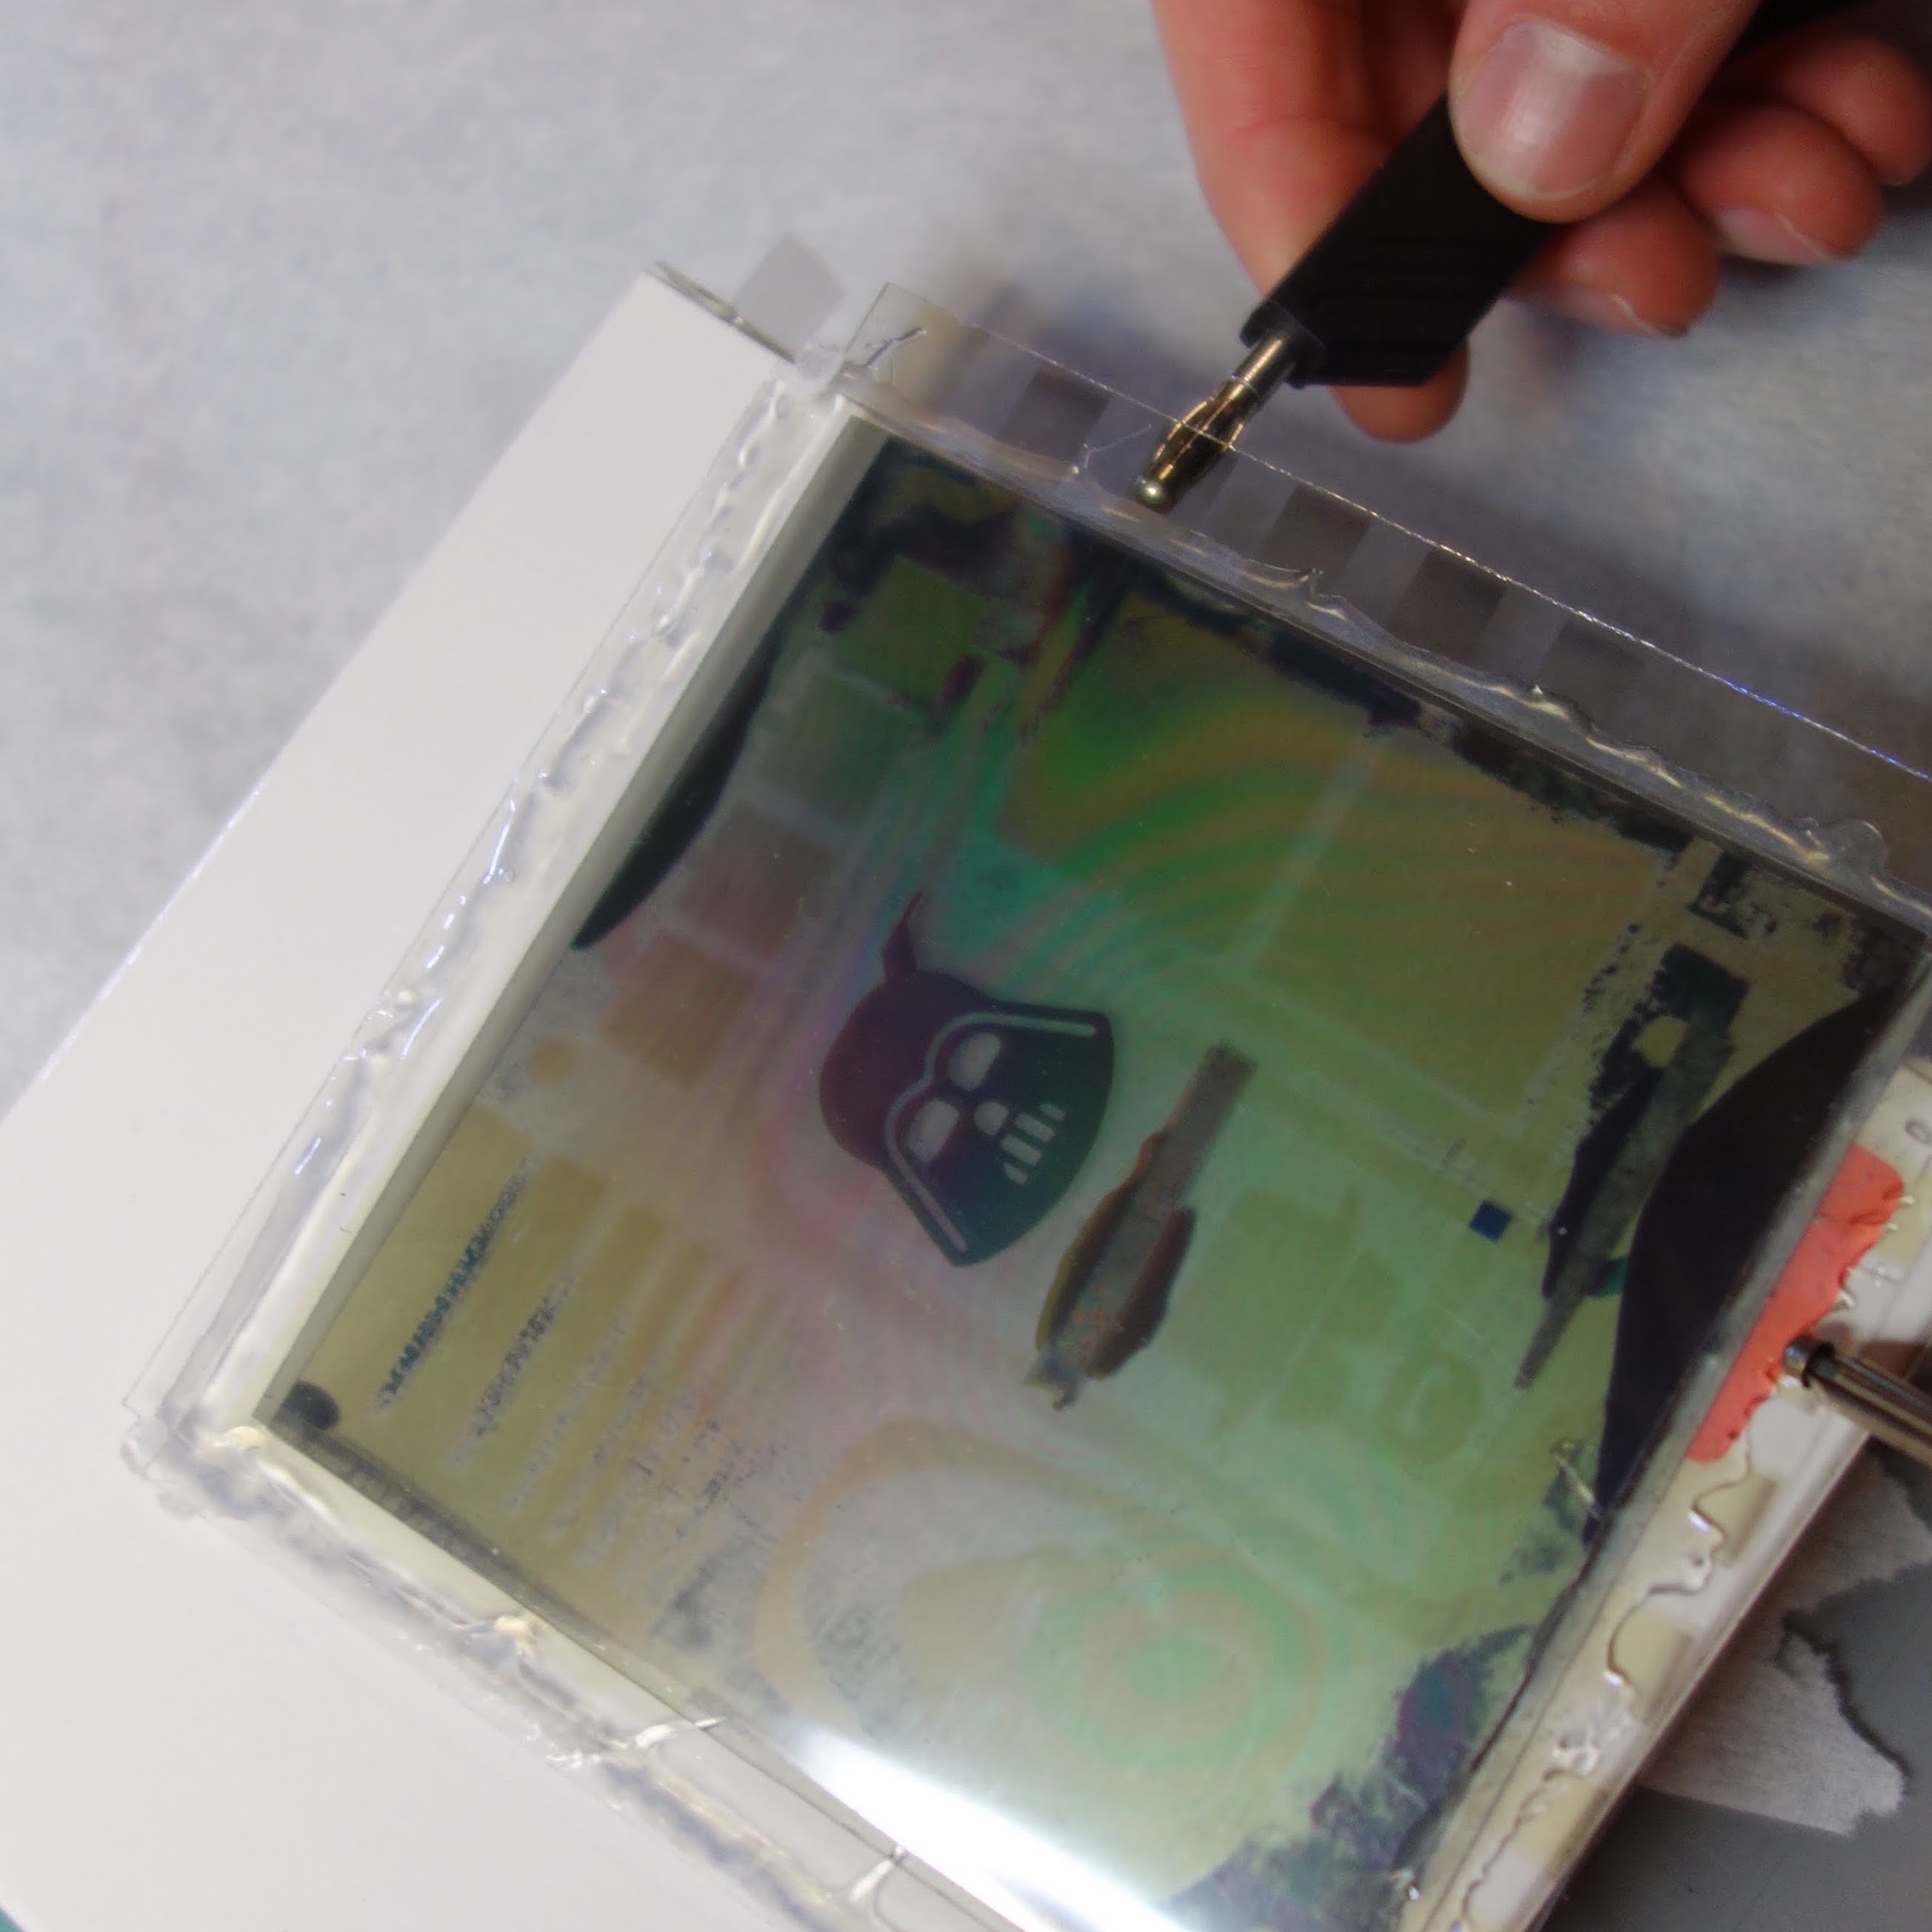
\includegraphics[width=0.22\textwidth]{./Bilder/DarthLeuchtet.jpg}
	}
    \caption{Produktionsschritte bei LCD-Herstellung}
\end{figure}
